% ============================================================================
%  BÁO CÁO ĐỒ ÁN MÔN HỌC — CS106 Trí tuệ nhân tạo
%  Đề tài 4: Xây dựng hệ thống tra cứu kiến thức pháp luật
%            (lĩnh vực giao thông đường bộ)
%  Biên dịch:  latexmk -xelatex main.tex
%
%  Định dạng theo hướng dẫn của đề (De_bai/Huong_dan_viet_bao_cao_Word):
%  Times New Roman 14 · lề trên 2, dưới 2, trái 3, phải 2 (cm) · khổ đứng
%  · trang bìa có viền Box, cách chữ 1 pt trên/dưới và 4 pt trái/phải.
% ============================================================================
\documentclass[14pt,a4paper]{extarticle}

% ---------- Font & ngôn ngữ ----------
\usepackage{fontspec}
\setmainfont{Times New Roman}
\setsansfont{Arial}
\setmonofont{Courier New}[Scale=0.92]
\usepackage[vietnamese]{babel}

% ---------- Trang ----------
\usepackage[a4paper,top=2cm,bottom=2cm,left=3cm,right=2cm,
            headheight=17pt,headsep=0.35cm,footskip=0.9cm]{geometry}
\usepackage{setspace}
\setstretch{1.18}
\setlength{\parskip}{0.3em}
\setlength{\parindent}{0pt}
\usepackage{microtype}
\setlength{\emergencystretch}{3em}
\usepackage{fancyhdr}
\usepackage{titlesec}
\usepackage{enumitem}
\setlist{itemsep=0.2em,topsep=0.3em,leftmargin=1.4em}

% ---------- Toán, bảng, hình ----------
\usepackage{amsmath}
\usepackage{unicode-math}
\setmathfont{texgyretermes-math.otf}
\usepackage{booktabs,tabularx,multirow,array,longtable}
\usepackage{graphicx}
\usepackage[table]{xcolor}
\usepackage{caption}
\captionsetup{font=small,labelfont=bf,labelsep=period,justification=centering}
\captionsetup[table]{position=top,skip=4pt}
\usepackage{float}
\usepackage[section]{placeins}
\usepackage{pifont}
\usepackage{tikz}
\usetikzlibrary{calc}
\usepackage[most]{tcolorbox}
\usepackage{listings}
\usepackage[ruled,vlined,linesnumbered]{algorithm2e}
\usepackage{hyperref}
\hypersetup{colorlinks=true,linkcolor=black,citecolor=uitblue,urlcolor=uitblue,
  pdftitle={CS106 - De tai 4 - He thong tra cuu kien thuc phap luat giao thong duong bo},
  pdfauthor={Nhom 7 - CS106.F31.CN2}}

% ---------- Màu & hộp nhấn mạnh ----------
\definecolor{uitblue}{HTML}{1F4E8C}
\definecolor{softgray}{HTML}{F3F4F6}
\definecolor{warnorange}{HTML}{A15A00}
\definecolor{okgreen}{HTML}{2E7D32}
\definecolor{badred}{HTML}{B3261E}
\newtcolorbox{keybox}[1][]{enhanced,breakable,colback=softgray,colframe=uitblue,
  boxrule=0pt,leftrule=3pt,arc=0pt,left=8pt,right=8pt,top=5pt,bottom=5pt,#1}
\newtcolorbox{warnbox}[1][]{enhanced,breakable,colback=orange!6,colframe=warnorange,
  boxrule=0pt,leftrule=3pt,arc=0pt,left=8pt,right=8pt,top=5pt,bottom=5pt,#1}

\lstset{basicstyle=\ttfamily\footnotesize,columns=fullflexible,keepspaces=true,
  frame=single,rulecolor=\color{black!20},backgroundcolor=\color{softgray},
  numbers=none,breaklines=true,showstringspaces=false,extendedchars=true,
  xleftmargin=4pt,xrightmargin=4pt,aboveskip=6pt,belowskip=6pt}

% ---------- Tiêu đề mục ----------
\titleformat{\section}{\normalfont\Large\bfseries}{\thesection.}{0.6em}{}
\titleformat{\subsection}{\normalfont\large\bfseries}{\thesubsection.}{0.6em}{}
\titleformat{\subsubsection}{\normalfont\normalsize\bfseries}{\thesubsubsection.}{0.6em}{}
\titlespacing*{\section}{0pt}{0pt}{1.0em}
\titlespacing*{\subsection}{0pt}{1.0em}{0.4em}
\titlespacing*{\subsubsection}{0pt}{0.8em}{0.3em}
\setcounter{secnumdepth}{3}
\setcounter{tocdepth}{2}
\newcommand{\sectionbreak}{\clearpage}

% ---------- Thuật ngữ trong algorithm2e ----------
\SetKwInput{KwIn}{Đầu vào}
\SetKwInput{KwOut}{Đầu ra}
\SetAlgorithmName{Thuật giải}{thuật giải}{Danh sách thuật giải}
\SetKwFor{ForEach}{với mỗi}{thực hiện}{hết}
\SetKwFor{While}{trong khi}{thực hiện}{hết}
\SetKwIF{If}{ElseIf}{Else}{nếu}{thì}{ngược lại nếu}{ngược lại}{hết}
\SetKw{Return}{trả về}

% ---------- Tiện ích ----------
\newcommand{\code}[1]{{\small\texttt{#1}}}
\newcommand{\dat}{\textcolor{okgreen}{\ding{51}}}
\newcolumntype{R}{>{\raggedleft\arraybackslash}X}
\newcolumntype{L}{>{\raggedright\arraybackslash}X}
\newcolumntype{C}{>{\centering\arraybackslash}X}

% ---------- Tên gọi tiếng Việt ----------
\addto\captionsvietnamese{%
  \renewcommand{\contentsname}{Mục lục}%
  \renewcommand{\listfigurename}{Danh sách hình}%
  \renewcommand{\listtablename}{Danh sách bảng}%
  \renewcommand{\refname}{Tài liệu tham khảo}%
  \renewcommand{\figurename}{Hình}%
  \renewcommand{\tablename}{Bảng}}

% ---------- Header / footer ----------
\pagestyle{fancy}
\fancyhf{}
\fancyhead[L]{\footnotesize\color{black!60}CS106 --- Trí tuệ nhân tạo}
\fancyhead[R]{\footnotesize\color{black!60}Đề tài 4 --- Tra cứu pháp luật giao thông đường bộ}
\fancyfoot[C]{\small\thepage}
\renewcommand{\headrulewidth}{0.4pt}
\fancypagestyle{plain}{\fancyhf{}\fancyfoot[C]{\small\thepage}\renewcommand{\headrulewidth}{0pt}}

\begin{document}

% ============================================================================
%  TRANG BÌA — viền Box theo hướng dẫn: cách vùng chữ 1 pt trên/dưới, 4 pt trái/phải
% ============================================================================
\begin{titlepage}
\begin{tikzpicture}[remember picture,overlay]
  \draw[line width=1.6pt]
    ($(current page.north west)+(3cm-4pt,-2cm+1pt)$) rectangle
    ($(current page.south east)+(-2cm+4pt,2cm-1pt)$);
  \draw[line width=0.5pt]
    ($(current page.north west)+(3cm-1pt,-2cm-2pt)$) rectangle
    ($(current page.south east)+(-2cm+1pt,2cm+2pt)$);
\end{tikzpicture}\par
\centering
\vspace*{0.35cm}
{\normalsize\bfseries ĐẠI HỌC QUỐC GIA THÀNH PHỐ HỒ CHÍ MINH\par}
{\normalsize\bfseries TRƯỜNG ĐẠI HỌC CÔNG NGHỆ THÔNG TIN\par}
{\normalsize\bfseries KHOA KHOA HỌC MÁY TÍNH\par}
\vspace{0.5cm}

\includegraphics[width=3.2cm]{figures/uit_logo.png}\par
\vspace{0.5cm}
{\large\bfseries CS106 --- TRÍ TUỆ NHÂN TẠO\par}
\vspace{0.3cm}
{\normalsize BÁO CÁO ĐỒ ÁN MÔN HỌC\par}
\vspace{0.5cm}
{\large\bfseries ĐỀ TÀI 4\par}
\vspace{0.2cm}
{\LARGE\bfseries XÂY DỰNG HỆ THỐNG TRA CỨU\\[3pt] KIẾN THỨC PHÁP LUẬT\par}
\vspace{0.25cm}
{\normalsize\itshape Lĩnh vực: Giao thông đường bộ\par}
\vspace{0.5cm}
{\normalsize
\begin{tabular}{@{}l l@{}}
Giảng viên hướng dẫn: & \textbf{PGS.TS. Nguyễn Đình Hiển} \\
Lớp: & \textbf{CS106.F31.CN2} \qquad Nhóm: \textbf{7} \\
\end{tabular}\par}
\vspace{0.35cm}
{\small
\renewcommand{\arraystretch}{1.08}
\begin{tabular}{c l c}
\toprule
\textbf{STT} & \textbf{Họ và tên} & \textbf{MSSV} \\
\midrule
1 & Nguyễn Quang Lâm & 25210289 \\
2 & Trần Trọng Tấn   & 25210334 \\
3 & Lê Quang Thi     & 25210337 \\
4 & Vỏ Cẩm Thu       & 25210342 \\
5 & Nguyễn Trí Toàn  & 26410135 \\
6 & Nguyễn Văn Thái  & 26410108 \\
7 & Đỗ Quốc Hoàng    & 26410043 \\
\bottomrule
\end{tabular}\par}
\vfill
{\normalsize\itshape Thành phố Hồ Chí Minh, tháng 9 năm 2026\par}
\vspace*{0.45cm}
\end{titlepage}

% ============================================================================
\pagenumbering{roman}
% ============================================================================
%  PHẦN ĐẦU: Lời cảm ơn · Tóm tắt · Mục lục · Danh sách hình/bảng · Từ viết tắt
% ============================================================================

\section*{Lời cảm ơn}
\addcontentsline{toc}{section}{Lời cảm ơn}

Nhóm 7 xin gửi lời cảm ơn chân thành đến PGS.TS. Nguyễn Đình Hiển, giảng viên môn
\emph{Trí tuệ nhân tạo} (CS106), đã giới thiệu các phương pháp biểu diễn tri thức và suy
diễn làm nền tảng cho đồ án, cũng như dòng nghiên cứu mô hình tri thức cho văn bản pháp
luật mà hệ thống của nhóm kế thừa.

Nhóm cũng cảm ơn cộng đồng mã nguồn mở Python, scikit-learn, FastAPI và Pydantic đã cung
cấp hạ tầng để một nhóm sinh viên có thể xây dựng, kiểm thử và đóng gói trọn vẹn một hệ
tra cứu pháp luật chạy được trên máy tính cá nhân.

\vspace{1em}
\hfill Thành phố Hồ Chí Minh, tháng 9 năm 2026

\hfill Nhóm 7

\clearpage
% ----------------------------------------------------------------------------
\section*{Tóm tắt}
\addcontentsline{toc}{section}{Tóm tắt}

Đồ án xây dựng một \textbf{hệ thống tra cứu kiến thức pháp luật giao thông đường bộ}
theo khung pháp lý 2024--2026, gồm Luật Trật tự, an toàn giao thông đường bộ số
36/2024/QH15, Nghị định 168/2024/NĐ-CP và hai văn bản sửa đổi là Luật 118/2025/QH15 và
Nghị định 238/2026/NĐ-CP. Khác với hướng truy hồi văn bản hay sinh câu trả lời bằng mô
hình ngôn ngữ lớn, hệ thống biểu diễn tri thức \emph{tường minh} bằng mô hình
$K = (C, R, \mathit{Rules}, F, \mathit{Keyphrase})$ và \emph{không sinh ngôn ngữ tự
nhiên}: mọi câu trả lời đều là nguyên văn điều khoản kèm căn cứ tới mức điều -- khoản --
điểm.

Cơ sở tri thức gồm 73 khái niệm, 482 quan hệ, 109 quy tắc, 345 hành vi vi phạm và 1.674
cụm từ khoá; 100\% mục tri thức có căn cứ pháp lý và khoảng hiệu lực, 63 sửa đổi được lưu
như dữ liệu để trả lời được câu hỏi ``tại thời điểm $t$ thì áp dụng quy định nào''. Thuật
giải xử lý truy vấn sáu bước (B1--B6) phân loại câu hỏi vào bảy lớp bài toán, xếp hạng tri
thức bằng hàm điểm lai ba thành phần (keyphrase, ngữ nghĩa TF-IDF, ngữ cảnh) và dùng bộ
suy diễn số học để chọn đúng khung phạt theo ngưỡng nồng độ cồn, tốc độ.

Trên bộ đánh giá 120 câu hỏi có đáp án chuẩn gán tới định danh tri thức, hệ thống đạt độ
chính xác phân lớp \textbf{95,83\%}, \textbf{Top-1 76,67\%} (khoảng tin cậy 95\%:
68,3--83,3\%), Top-5 95,00\% và MRR 0,8384, với thời gian trả lời trung bình 6,2~ms. Thí
nghiệm loại bỏ thành phần cho thấy suy diễn số học nâng Top-1 của nhóm câu có giá trị số
từ 40,9\% lên 95,5\%, và kiểm định McNemar ($p = 0{,}000488$) khẳng định cải thiện này có ý
nghĩa thống kê. Mọi hạn chế --- trong đó có việc cấu hình mặc định chưa từ chối được truy
vấn ngoài lĩnh vực --- đều được đo và khoá lại bằng kiểm thử. Toàn bộ số liệu tái lập được
bằng một lệnh chạy.

\vspace{0.6em}
\noindent\textbf{Từ khoá:} biểu diễn tri thức, hệ tra cứu pháp luật, giao thông đường bộ,
keyphrase, suy diễn số học, hiệu lực theo thời gian, tiếng Việt.

\clearpage
% ----------------------------------------------------------------------------
{\setstretch{1.05}
\tableofcontents
\clearpage
\listoffigures
\addcontentsline{toc}{section}{Danh sách hình}
\vspace{1.2em}
\listoftables
\addcontentsline{toc}{section}{Danh sách bảng}
}

\clearpage
% ----------------------------------------------------------------------------
\section*{Danh mục từ viết tắt}
\addcontentsline{toc}{section}{Danh mục từ viết tắt}

\begin{center}
\renewcommand{\arraystretch}{1.15}
\begin{tabularx}{\textwidth}{@{}l L@{}}
\toprule
\textbf{Viết tắt} & \textbf{Ý nghĩa} \\
\midrule
GTĐB      & Giao thông đường bộ \\
GPLX      & Giấy phép lái xe \\
NĐ-CP     & Nghị định của Chính phủ \\
QH        & Luật do Quốc hội ban hành \\
VBHN-VPQH & Văn bản hợp nhất của Văn phòng Quốc hội \\
KB        & Knowledge Base --- cơ sở tri thức \\
TF-IDF    & Term Frequency -- Inverse Document Frequency \\
MRR       & Mean Reciprocal Rank --- hạng nghịch đảo trung bình \\
KTC       & Khoảng tin cậy \\
AUC       & Area Under the ROC Curve --- diện tích dưới đường cong ROC \\
RAG       & Retrieval-Augmented Generation --- sinh văn bản có truy hồi \\
LLM       & Large Language Model --- mô hình ngôn ngữ lớn \\
API       & Application Programming Interface \\
CI        & Continuous Integration --- tích hợp liên tục \\
xfail     & Kiểm thử được đánh dấu ``dự kiến thất bại'' kèm số đo hạn chế \\
\bottomrule
\end{tabularx}
\end{center}


\clearpage
\pagenumbering{arabic}
% ============================================================================
%  1. TỔNG QUAN
% ============================================================================
\section{Tổng quan}
\label{sec:tong-quan}

\subsection{Bối cảnh và động lực}

Luật Trật tự, an toàn giao thông đường bộ số 36/2024/QH15~\cite{luat36} và Nghị định
168/2024/NĐ-CP~\cite{nd168} cùng có hiệu lực từ ngày 01 tháng 01 năm 2025, thay thế toàn bộ
khung pháp lý cũ và nâng mạnh mức xử phạt ở nhiều nhóm hành vi. Chỉ trong hơn một năm sau
đó, khung này tiếp tục được sửa đổi hai lần: Luật 118/2025/QH15~\cite{luat118} (hiệu lực
01/7/2026) và Nghị định 238/2026/NĐ-CP~\cite{nd238} (hiệu lực 15/8/2026). Người tham gia giao
thông vì vậy đứng trước một khối văn bản vừa mới, vừa phân tán, vừa liên tục thay đổi.

Khó khăn thực tế không nằm ở chỗ thiếu thông tin mà ở chỗ thông tin bị \emph{tách rời}.
Luật quy định hành vi nào bị nghiêm cấm; nghị định mới quy định hành vi đó bị phạt bao
nhiêu tiền và bị trừ mấy điểm giấy phép lái xe. Câu hỏi thường gặp nhất của người dân ---
\emph{``vượt đèn đỏ phạt bao nhiêu''} --- do đó không thể trả lời nếu chỉ đọc một văn bản.
Các công cụ tìm kiếm phổ thông trả về toàn văn điều khoản, buộc người hỏi tự đối chiếu;
còn các trợ lý sinh ngôn ngữ tự nhiên thì có nguy cơ diễn giải sai lời của luật mà không
nêu được căn cứ.

Một câu trả lời sai trong tra cứu pháp luật không phải là ``kết quả kém hơn một chút'' mà
là thông tin dẫn người dân tới hành vi sai. Ba đặc điểm của lĩnh vực giao thông đường bộ
khiến nó đặc biệt phù hợp với hướng \textbf{tri thức tường minh}:
\begin{itemize}
  \item văn bản có cấu trúc chặt (điều -- khoản -- điểm) nên mô hình hoá được;
  \item tri thức mang tính \emph{suy diễn số} (ngưỡng nồng độ cồn, mức vượt tốc độ, điểm
        trừ cộng dồn) nên so khớp văn bản đơn thuần là không đủ;
  \item mọi câu trả lời đều phải truy nguyên được về một căn cứ pháp lý cụ thể.
\end{itemize}

\subsection{Phát biểu bài toán}
\label{sec:phat-bieu}

Cho cơ sở tri thức
\begin{equation}
  K = (C,\; R,\; \mathit{Rules},\; F,\; \mathit{Keyphrase})
  \label{eq:K}
\end{equation}
trong đó $C$ là tập khái niệm pháp lý, $R \subseteq C \times C$ là tập quan hệ hai ngôi,
$\mathit{Rules}$ là tập quy tắc giao thông, $F$ là tập sự kiện ``hành vi vi phạm -- chế
tài'', và $\mathit{Keyphrase}$ là từ điển cụm từ khoá ánh xạ ngôn ngữ người dùng vào định
danh tri thức. Mỗi phần tử tri thức $x$ mang một khối căn cứ
$cc(x) = (\text{văn bản}, \text{điều}, \text{khoản}, \text{điểm})$ và một khoảng hiệu lực
$hl(x) = [t_{\text{bắt đầu}},\, t_{\text{kết thúc}})$.

\begin{table}[H]
\centering
\caption{Định nghĩa hình thức đầu vào -- đầu ra của bài toán}
\label{tab:io}
\renewcommand{\arraystretch}{1.3}
\begin{tabularx}{\textwidth}{@{}>{\bfseries}p{2.7cm} L@{}}
\toprule
Thành phần & \textbf{Định nghĩa} \\
\midrule
Đầu vào & Truy vấn $q$ là chuỗi tiếng Việt tự nhiên (có dấu hoặc không dấu), kèm tuỳ chọn
mốc thời gian $t$ (mặc định: ngày hiện tại) và bộ lọc phương tiện. \\
Đầu ra & Bộ ba $A(q,t) = (p, T, E)$: $p \in \{P1,\dots,P7\}$ là lớp bài toán được nhận
diện; $T \subseteq C \cup \mathit{Rules} \cup F$ là danh sách tối đa $k$ mẩu tri thức đã
xếp hạng, mọi $x \in T$ đều thoả $t \in hl(x)$; $E$ là phần giải trình gồm nguyên văn điều
khoản và căn cứ $cc(x)$ của từng $x \in T$. \\
Ràng buộc & Hệ thống \emph{không} sinh ngôn ngữ tự nhiên: mọi câu chữ trong $E$ đều là
trích nguyên văn từ văn bản nguồn. Nếu không có $x$ nào thoả, hệ trả về tập rỗng kèm lý do
chứ không suy đoán. \\
Mục tiêu & Cực đại hoá xác suất đáp án chuẩn nằm ở hạng 1 của $T$ (Top-1) và nằm trong $T$
(Top-$k$), đồng thời giữ độ chính xác phân lớp $p$ và bảo đảm 100\% phần tử trả về truy
nguyên được căn cứ. \\
\bottomrule
\end{tabularx}
\end{table}

Phát biểu này tách bạch hai việc thường bị gộp làm một trong các hệ hỏi đáp: \textbf{tìm
đúng} mẩu tri thức ($T$) và \textbf{giải trình được} vì sao ($E$). Hệ thống bị ràng buộc
phải làm được cả hai, và chính ràng buộc ``không sinh ngôn ngữ'' là thứ phân biệt đồ án với
hướng RAG/LLM trình bày ở mục~\ref{sec:lien-quan}.

\subsection{Đóng góp của nhóm}

\begin{enumerate}
  \item \textbf{Cơ sở tri thức mở} cho lĩnh vực giao thông đường bộ theo khung pháp lý
        2024--2026: 73 khái niệm, 482 quan hệ, 109 quy tắc, 345 hành vi vi phạm và 1.674
        cụm từ khoá; 100\% mục có căn cứ pháp lý ở mức điều -- khoản -- điểm và có khoảng
        hiệu lực.
  \item \textbf{Mô hình hoá hiệu lực theo thời gian ở mức khoản}: sửa đổi được lưu như dữ
        liệu (63 bản ghi) chứ không hợp nhất cứng, nhờ đó trả lời được câu hỏi ``tại thời
        điểm $t$ thì áp dụng quy định nào''.
  \item \textbf{Thuật giải xử lý truy vấn sáu bước} với hàm điểm lai ba thành phần và bộ
        suy diễn số học cho các điều khoản phân khung theo ngưỡng; thí nghiệm loại bỏ thành
        phần chứng minh từng thành phần đều đóng góp thực chất.
  \item \textbf{Bộ dữ liệu đánh giá} 120 câu hỏi có đáp án chuẩn gán tới mức định danh tri
        thức, 40 truy vấn ngoài lĩnh vực, cùng toàn bộ kết quả đo, kiểm định thống kê và
        phân tích lỗi tái lập được bằng một lệnh chạy.
\end{enumerate}

\subsection{Cấu trúc báo cáo}

Mục~\ref{sec:lien-quan} khảo sát các công trình liên quan và xác định khoảng trống.
Mục~\ref{sec:du-lieu} trình bày cách xây dựng và phân tích bộ dữ liệu.
Mục~\ref{sec:phuong-phap} mô tả kiến trúc, thuật giải và thiết lập thực nghiệm.
Mục~\ref{sec:ket-qua} báo cáo kết quả, kiểm định thống kê và phân tích lỗi.
Mục~\ref{sec:ket-luan} trình bày ứng dụng, hạn chế, hướng phát triển và kết luận.
Phụ lục~A ghi phân công công việc; Phụ lục~B liệt kê các lệnh kiểm chứng lại số liệu.

% ============================================================================
%  2. CÁC CÔNG TRÌNH LIÊN QUAN
% ============================================================================
\section{Các công trình liên quan}
\label{sec:lien-quan}

\subsection{Khảo sát các hướng tiếp cận hiện tại}

Các công trình về hỏi đáp và truy hồi văn bản pháp luật có thể xếp vào bốn hướng, khác
nhau ở chỗ \emph{tri thức pháp lý nằm ở đâu}.

\subsubsection{Hướng 1 --- Truy hồi ngữ nghĩa bằng mạng nơ-ron}

Tri thức nằm trong tham số của mô hình ngôn ngữ. PhoBERT~\cite{phobert} là xương sống cho
phần lớn hệ truy hồi luật tiếng Việt; Pham và cộng sự~\cite{phamMultistage} đề xuất truy
hồi nhiều giai đoạn cho văn bản luật tiếng Việt; Tiên và cộng sự~\cite{tienSynthetic} dùng
dữ liệu tổng hợp do mô hình lớn sinh ra để khắc phục khan hiếm nhãn. Ở quy mô quốc tế,
LEGAL-BERT~\cite{legalbert} cho thấy tiếp tục tiền huấn luyện theo miền pháp luật cải thiện
rõ các tác vụ pháp lý, còn Nguyen và cộng sự~\cite{nguyenAttentive} đưa kiến trúc chú ý
phân cấp cho văn bản luật dài. Điểm chung: đầu ra là một \emph{đoạn văn bản} được xếp hạng,
không phải tri thức có cấu trúc, nên hệ thống không giải thích được vì sao điều khoản đó áp
dụng và không tính được mức phạt.

\subsubsection{Hướng 2 --- Ontology và đồ thị tri thức pháp luật}

Tri thức được mô hình hoá tường minh. Legal-Onto~\cite{legalonto} đề xuất mô hình tri thức
gồm khái niệm có cấu trúc, ba loại quan hệ, luật suy diễn và đồ thị cụm từ khoá, áp dụng
cho Luật Đất đai; đây chính là dòng nghiên cứu mà mô hình $K$ của đồ án kế thừa, cùng với
nền tảng Rela-model~\cite{relamodel} và COKB~\cite{cokb}. Các mở rộng sau đó phủ thêm luật
lao động~\cite{phamLabor,phamLegalOntoUpdate}, tích hợp ontology với đồ thị tri thức cho
truy vấn pháp lý~\cite{phamOntoKG}, và gần đây là kiến trúc ontology ba tầng đa
miền~\cite{phamUnified}. Đáng chú ý nhất với đồ án là Dang và cộng sự~\cite{dangKG} ---
công trình đồ thị tri thức cho chính luật giao thông đường bộ Việt Nam, nhưng dựa trên Luật
23/2008/QH12 đã hết hiệu lực.

\subsubsection{Hướng 3 --- RAG và mô hình ngôn ngữ lớn cho miền pháp luật}

Đây là hướng phổ biến nhất hiện nay, và cũng là hướng nhóm \emph{chủ động không chọn}. Dahl
và cộng sự~\cite{dahl} đo được LLM đa dụng bịa căn cứ pháp lý một cách có hệ thống; Magesh
và cộng sự~\cite{magesh} đánh giá tiền đăng ký các công cụ RAG pháp lý thương mại và ghi
nhận tỉ lệ ảo giác 17--33\% dù nhà cung cấp quảng cáo ``hallucination-free''; benchmark
ALCE~\cite{alce} cho thấy trích dẫn do mô hình sinh thường không trung thực với nguồn. Ngay
cả các hệ kết hợp đồ thị tri thức với RAG cho luật Việt Nam~\cite{phamKGRAG,laura} vẫn giữ
mô hình sinh ở khâu cuối, nên vẫn thừa hưởng rủi ro này.

\subsubsection{Hướng 4 --- Hiệu lực theo thời gian của quy phạm}

Lý thuyết đã tương đối đầy đủ ở quốc tế: Governatori và cộng sự~\cite{governatori} hình
thức hoá ba loại sửa đổi (thay thế, bãi bỏ một phần, huỷ bỏ hồi tố) bằng logic khả bác có
gắn thời gian; Palmirani và cộng sự~\cite{palmirani} quản lý tiến hoá văn bản theo ba chiều
hiệu lực; chuẩn LegalRuleML~\cite{legalruleml} đưa toán tử nghĩa vụ cùng chiều thời gian vào
biểu diễn; de Martim~\cite{demartim} tách tác phẩm trừu tượng khỏi biểu hiện có phiên bản để
trả lời tất định câu hỏi ``văn bản tại thời điểm $t$''. Phía Việt Nam, Pham và cộng
sự~\cite{phamLegalOntoUpdate} mới dừng ở đối sánh hai phiên bản Luật Đất đai 2013 và 2024
--- tức phát hiện thay đổi, chưa phải truy vấn theo mốc thời gian.

\subsection{Các bộ dữ liệu đã có}

\begin{table}[H]
\centering
\caption{Các bộ dữ liệu hỏi đáp và truy hồi pháp luật tiêu biểu}
\label{tab:datasets}
\small
\renewcommand{\arraystretch}{1.25}
\begin{tabularx}{\textwidth}{@{}>{\raggedright\arraybackslash}p{3.1cm} >{\raggedright\arraybackslash}p{3.0cm} L L@{}}
\toprule
\textbf{Bộ dữ liệu} & \textbf{Ngôn ngữ · miền} & \textbf{Quy mô} & \textbf{Nhiệm vụ} \\
\midrule
VLQA / DRILL~\cite{vlqa,drill} & Tiếng Việt · 27 lĩnh vực & 3.129 câu hỏi · 59.636 điều luật của 2.162 văn bản & Truy hồi điều luật và sinh câu trả lời có trích dẫn \\
MLQA-TSR, VLSP 2025~\cite{mlqatsr} & Tiếng Việt · biển báo GTĐB & 776 câu hỏi · 402 điều · 498 ảnh biển báo & Truy hồi và hỏi đáp đa phương thức ảnh -- văn bản \\
ALQAC~\cite{alqac} & Tiếng Việt (và tiếng Thái) & Chưa kiểm chứng từ nguồn chính thức & Truy hồi văn bản luật, suy luận kéo theo, hỏi đáp \\
Zalo AI Challenge 2021~\cite{zalo} & Tiếng Việt · văn bản luật & Chưa kiểm chứng từ nguồn chính thức & Truy hồi văn bản luật (Acc@1) \\
COLIEE~\cite{coliee} & Tiếng Nhật / Anh · dân sự, án lệ & 768 điều Bộ luật Dân sự Nhật (Task 3--4) & Truy hồi luật thành văn và kiểm tra kéo theo \\
\midrule
\textbf{Bộ dữ liệu của nhóm} & Tiếng Việt · GTĐB 2024--2026 & 120 câu hỏi · 345 hành vi · 109 quy tắc · 73 khái niệm & Tra cứu tri thức 7 lớp, gán nhãn tới \emph{định danh} tri thức \\
\bottomrule
\end{tabularx}
\end{table}

Bảng~\ref{tab:datasets} chỉ ghi con số khi kiểm chứng được từ bài báo hoặc trang chính thức;
các ô ``chưa kiểm chứng'' được để nguyên thay vì điền số ước đoán. Điểm cần lưu ý là
\textbf{đơn vị gán nhãn}: các bộ dữ liệu hiện có gán nhãn ở mức điều luật, trong khi bộ dữ
liệu của nhóm gán tới định danh của từng mẩu tri thức (một khái niệm, một quy tắc, một hành
vi kèm chế tài) --- nhờ vậy mới đo được Top-1 ở mức tri thức chứ không chỉ mức văn bản.

\subsection{Khoảng trống và chỗ đứng của đồ án}

Đối chiếu bốn hướng trên với yêu cầu Đề tài 4, nhóm xác định năm khoảng trống --- và đây
chính là chỗ đồ án đứng vào:

\begin{enumerate}
  \item \textbf{Chưa có hệ tra cứu tri thức cho GTĐB Việt Nam theo khung pháp lý 2024--2026.}
        Công trình đồ thị tri thức cùng miền gần nhất~\cite{dangKG} dựa trên Luật 23/2008 đã
        hết hiệu lực; MLQA-TSR~\cite{mlqatsr} tuy đúng khung luật mới nhưng giải bài toán
        nhận dạng biển báo đa phương thức, không phải tra cứu tri thức pháp lý.
  \item \textbf{Đầu ra là đoạn văn bản, không phải tri thức có cấu trúc.}
        VLQA/DRILL~\cite{vlqa,drill}, Zalo~\cite{zalo} và COLIEE Task~3~\cite{coliee} đều
        chấm ở mức ``xếp hạng điều luật đúng''; không nhiệm vụ nào yêu cầu trả về khái niệm,
        quan hệ và quy tắc suy diễn --- nên không đo được khả năng giải trình.
  \item \textbf{Chưa có công trình tiếng Việt kết hợp mô hình tri thức kiểu $K$ với suy diễn
        số học theo luật.} Legal-Onto~\cite{legalonto} và các mở
        rộng~\cite{phamLabor,phamLegalOntoUpdate,phamUnified} dừng ở tra cứu thuật ngữ và thủ
        tục, trong khi GTĐB đòi hỏi tính ra mức phạt tiền, thời hạn tước giấy phép và điểm
        trừ theo điều kiện phương tiện -- hành vi -- tình tiết.
  \item \textbf{Chưa mô hình hoá hiệu lực theo thời gian cho pháp luật Việt Nam.} Lý thuyết
        đã có~\cite{governatori,palmirani,legalruleml,demartim} nhưng phía Việt Nam mới dừng ở
        phát hiện thay đổi giữa hai phiên bản~\cite{phamLegalOntoUpdate}. Miền GTĐB thay đổi
        rất nhanh nên đây là khoảng trống có giá trị thực tiễn cao.
  \item \textbf{Hướng RAG/LLM chưa bảo đảm trung thực căn cứ} ở mức chấp nhận được cho tra
        cứu pháp luật~\cite{dahl,magesh,alce}. Đồ án chọn loại bỏ hoàn toàn khâu sinh, đổi độ
        ``mượt'' của câu trả lời lấy khả năng truy vết 100\% căn cứ --- một đánh đổi có chủ
        đích chứ không phải hạn chế kỹ thuật.
\end{enumerate}

% ============================================================================
%  3. XÂY DỰNG DỮ LIỆU
% ============================================================================
\section{Xây dựng dữ liệu}
\label{sec:du-lieu}

\subsection{Nguồn văn bản và giải trình phạm vi}

Đề bài yêu cầu chọn ``01 văn bản pháp luật tương ứng''. Nhóm thực hiện trên \textbf{bốn}
văn bản và xin giải trình ngay từ đầu, vì đây là quyết định thiết kế chứ không phải làm
lệch đề.

\begin{keybox}
Luật 36/2024/QH15 quy định \textbf{hành vi} nào bị nghiêm cấm nhưng không quy định mức phạt;
toàn bộ \textbf{chế tài} nằm ở Nghị định 168/2024/NĐ-CP. Nếu chỉ dùng văn bản luật gốc, hệ
thống sẽ không trả lời được câu hỏi phổ biến nhất trong thực tế là \emph{``phạt bao nhiêu
tiền''}. Hai văn bản sửa đổi được đưa thêm vào để hệ thống trả lời đúng \textbf{theo mốc thời
gian}, thay vì trả lời theo bản đã lỗi thời.
\end{keybox}

\begin{table}[H]
\centering
\caption{Bốn văn bản nguồn và vai trò trong cơ sở tri thức}
\label{tab:van-ban}
\renewcommand{\arraystretch}{1.2}
\begin{tabularx}{\textwidth}{@{}l L r@{}}
\toprule
\textbf{Văn bản} & \textbf{Vai trò} & \textbf{Hiệu lực} \\
\midrule
Luật 36/2024/QH15~\cite{luat36}        & Văn bản chính --- quy tắc, khái niệm, hành vi bị cấm & 01/01/2025 \\
Nghị định 168/2024/NĐ-CP~\cite{nd168}  & Văn bản chế tài --- mức phạt, trừ điểm GPLX          & 01/01/2025 \\
Luật 118/2025/QH15~\cite{luat118}      & Sửa đổi Luật 36/2024                                  & 01/7/2026 \\
Nghị định 238/2026/NĐ-CP~\cite{nd238}  & Sửa đổi Nghị định 168/2024                            & 15/8/2026 \\
\bottomrule
\end{tabularx}
\end{table}

Mọi mục tri thức đều được đối chiếu với Văn bản hợp nhất 55/VBHN-VPQH ngày
23/3/2026~\cite{vbhn55} của Văn phòng Quốc hội --- tức bản \emph{sau} sửa đổi. Trường
\code{can\_cu\_text} của từng bản ghi ghi rõ điều này, nên người chấm kiểm tra được ngay rằng
dữ liệu không phải bản cũ.

\subsection{Cấu trúc của cơ sở tri thức}

\begin{table}[H]
\centering
\caption{Năm thành phần của cơ sở tri thức $K$}
\label{tab:thanh-phan-K}
\renewcommand{\arraystretch}{1.2}
\begin{tabularx}{\textwidth}{@{}c l r L@{}}
\toprule
\textbf{Ký hiệu} & \textbf{Thành phần} & \textbf{Số lượng} & \textbf{Vai trò} \\
\midrule
$C$                 & Khái niệm        & 73    & Định nghĩa pháp lý --- ``xe cơ giới là gì'' \\
$R$                 & Quan hệ          & 482   & Đồ thị hai chiều nối các mảng tri thức \\
$\mathit{Rules}$    & Quy tắc          & 109   & Quy định phải làm / không được làm \\
$F$                 & Hành vi vi phạm  & 345   & Hành vi kèm chế tài: tiền, trừ điểm, hình phạt bổ sung \\
$\mathit{Keyphrase}$& Cụm từ khoá      & 1.674 & Cầu nối giữa ngôn ngữ người dùng và định danh tri thức \\
\bottomrule
\end{tabularx}
\end{table}

Ngoài năm thành phần trên, cơ sở tri thức còn lưu 4 bản ghi văn bản nguồn và \textbf{63 bản
ghi sửa đổi}. Sửa đổi được lưu như dữ liệu độc lập, không hợp nhất cứng lúc dựng cơ sở tri
thức --- nhờ vậy hệ thống trả lời được câu hỏi ``tại thời điểm nào thì quy định ra sao''.

\subsection{Cách lấy và chuẩn hoá dữ liệu}

\begin{itemize}
  \item \textbf{Trích xuất:} tách toàn văn theo cấu trúc điều -- khoản -- điểm từ bản công bố
        của bốn văn bản, lưu ở \code{data/raw/} dưới dạng JSON giữ nguyên văn. Không dùng bản
        tóm tắt hay bài viết lại của bên thứ ba.
  \item \textbf{Chuẩn hoá:} mỗi mục tri thức được gán một định danh ổn định (ví dụ
        \code{R01}, \code{VP\_OTO\_ND168D6\_K1A}), một khối căn cứ có cấu trúc và một khoảng
        hiệu lực. Chế tài được lưu \emph{có kiểu} --- số tiền và điểm trừ là số nguyên, không
        phải chuỗi --- nên cộng dồn và so sánh được.
  \item \textbf{Sinh keyphrase:} mỗi mục kèm danh sách cụm từ người dùng thật hay dùng, gồm
        cả khẩu ngữ (``nhậu'', ``vượt đèn đỏ'') và bản không dấu, để chịu được truy vấn gõ vội
        không dấu.
  \item \textbf{Kiểm toàn vẹn:} module \code{kb/validator.py} soát định danh trùng, quan hệ
        treo, keyphrase trỏ tới định danh không tồn tại và mục thiếu căn cứ. Toàn bộ kiểm tra
        này chạy trong CI, nên một bản ghi hỏng không thể lọt vào kho mã.
  \item \textbf{Xây bộ câu hỏi đánh giá:} mỗi câu được viết kèm đáp án chuẩn dạng văn bản,
        danh sách \emph{định danh} tri thức đúng, lớp bài toán đúng và mức độ khó. Có test kiểm
        chứng rằng mọi định danh trong đáp án chuẩn đều tồn tại trong cơ sở tri thức --- hiện
        120/120 câu đều chấm được, không có định danh treo.
\end{itemize}

Chuẩn hoá bằng mô hình có kiểu (Pydantic v2) chứ không phải \code{dict} tự do: trường lạ bị
từ chối ngay lúc nạp, nên một bản ghi sai cấu trúc không thể lọt vào cơ sở tri thức để đến
lúc chạy mới phát hiện. Một bản ghi hành vi vi phạm (rút gọn):

\begin{lstlisting}
{
  "id": "VP_OTO_ND168D6_K1A",
  "hanh_vi": "Không chấp hành hiệu lệnh, chỉ dẫn của biển báo hiệu,
              vạch kẻ đường, trừ ...",
  "nhom": "bien_bao_hieu",
  "phuong_tien": ["o_to"],
  "phat_tien": { "min": 400000, "max": 600000 },
  "tru_diem_gplx": 0,
  "can_cu": { "van_ban": "Nghị định 168/2024/NĐ-CP",
              "dieu": 6, "khoan": 1, "diem": "a" },
  "tinh_trang": "hien_hanh"
}
\end{lstlisting}

\subsection{Thống kê và phân tích bộ dữ liệu}

Ba phân bố dưới đây được sinh lại bằng một lệnh (xem Phụ lục~B) nên luôn khớp với dữ liệu thật trong kho mã, không phải số chép tay.

\subsubsection{Phân bố độ dài}

Câu hỏi dài trung bình \textbf{14,61 từ} (trung vị 14, ngắn nhất 3, dài nhất 38, độ lệch
chuẩn 6,10). Phân bố lệch phải rõ rệt: 75\% câu không quá 17 từ, nhưng đuôi kéo tới 38 từ --- đó
là các câu khẩu ngữ kể cả tình huống (\emph{``Nhóm em 4 đứa đi chung một xe máy, không ai đội
mũ bảo hiểm\dots''}). Đuôi này quan trọng: mục~\ref{sec:ket-qua} sẽ cho thấy phần lớn ca lỗi
nặng tập trung ở đó.

Về phía tri thức, hành vi vi phạm dài trung bình 42,0 từ và quy tắc dài trung bình 80,8 từ
--- dài gấp khoảng 5,5 lần câu hỏi. Đây là gốc rễ của bài toán: câu hỏi ngắn và đời thường
phải khớp với văn bản dài và trang trọng, nên chỉ so khớp bề mặt là không đủ.

\begin{figure}[H]
\centering
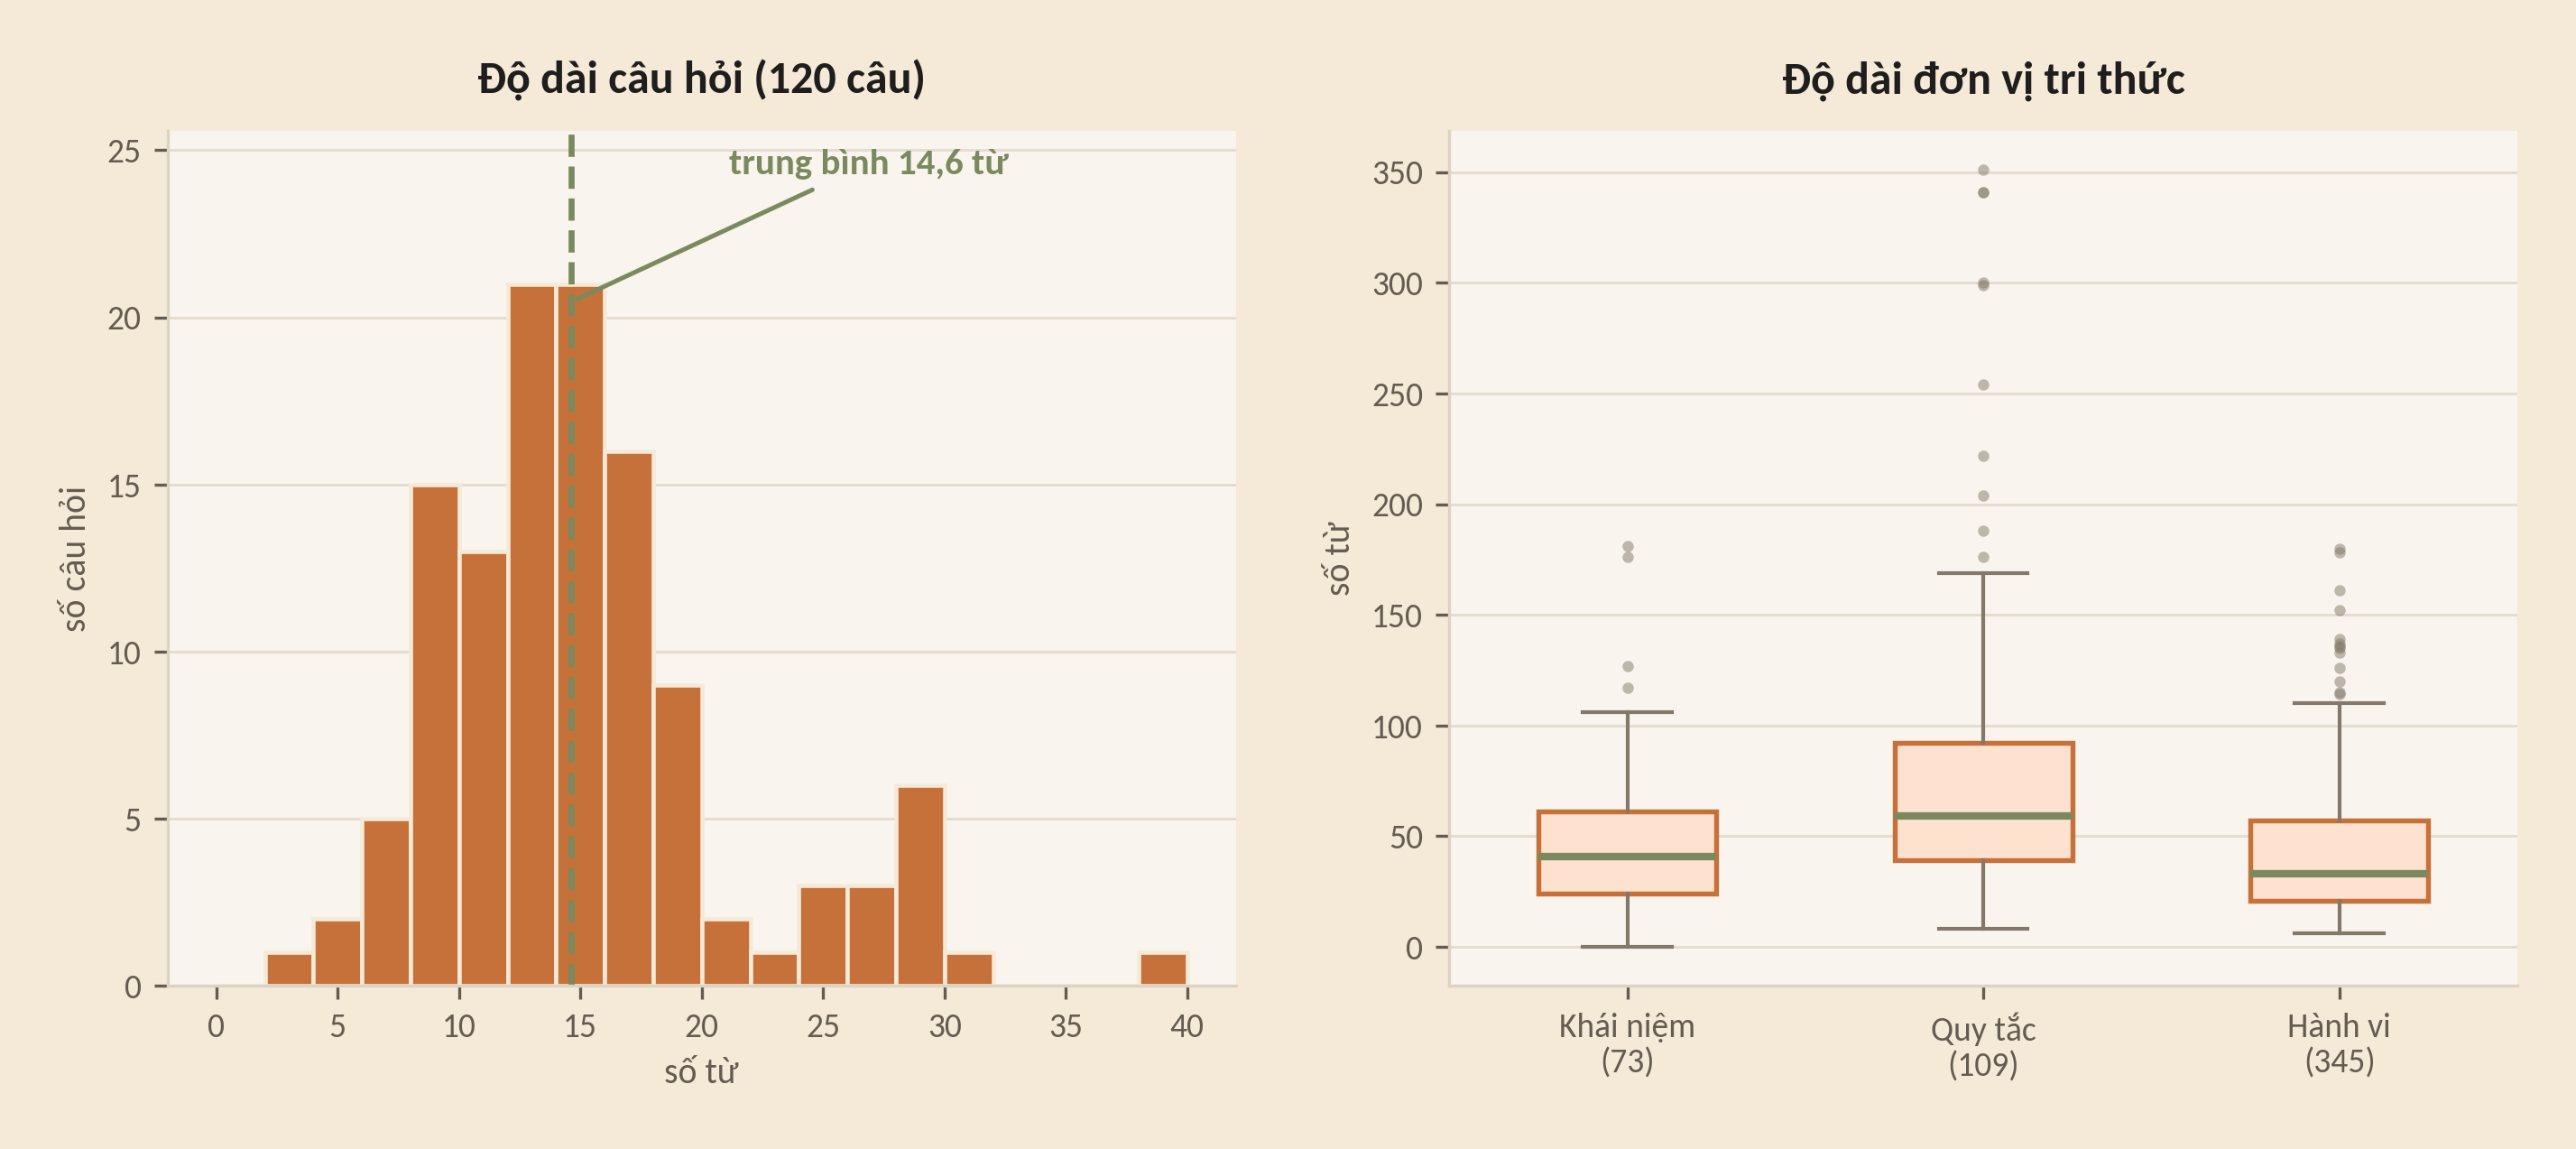
\includegraphics[width=\textwidth]{figures/hinh3_phan_bo_do_dai.png}
\caption{Phân bố độ dài câu hỏi và độ dài đơn vị tri thức}
\label{fig:do-dai}
\end{figure}

\subsubsection{Phân bố nhãn}

Bộ câu hỏi được phân bổ theo tần suất thực tế của nhu cầu tra cứu, không chia đều: lớp tra
cứu chế tài P3 chiếm 40/120 câu vì đây là câu hỏi người dân hỏi nhiều nhất. Về mức độ khó:
dễ 28 · trung bình 68 · khó 24. Về loại tri thức của đáp án chuẩn: khái niệm 22 · quy tắc 25
· hành vi vi phạm 73. Có \textbf{26/120 câu} có nhiều hơn một mẩu tri thức trong đáp án chuẩn
--- chi tiết này sẽ giải thích con số precision ở mục~\ref{sec:kiem-dinh}.

\begin{figure}[H]
\centering
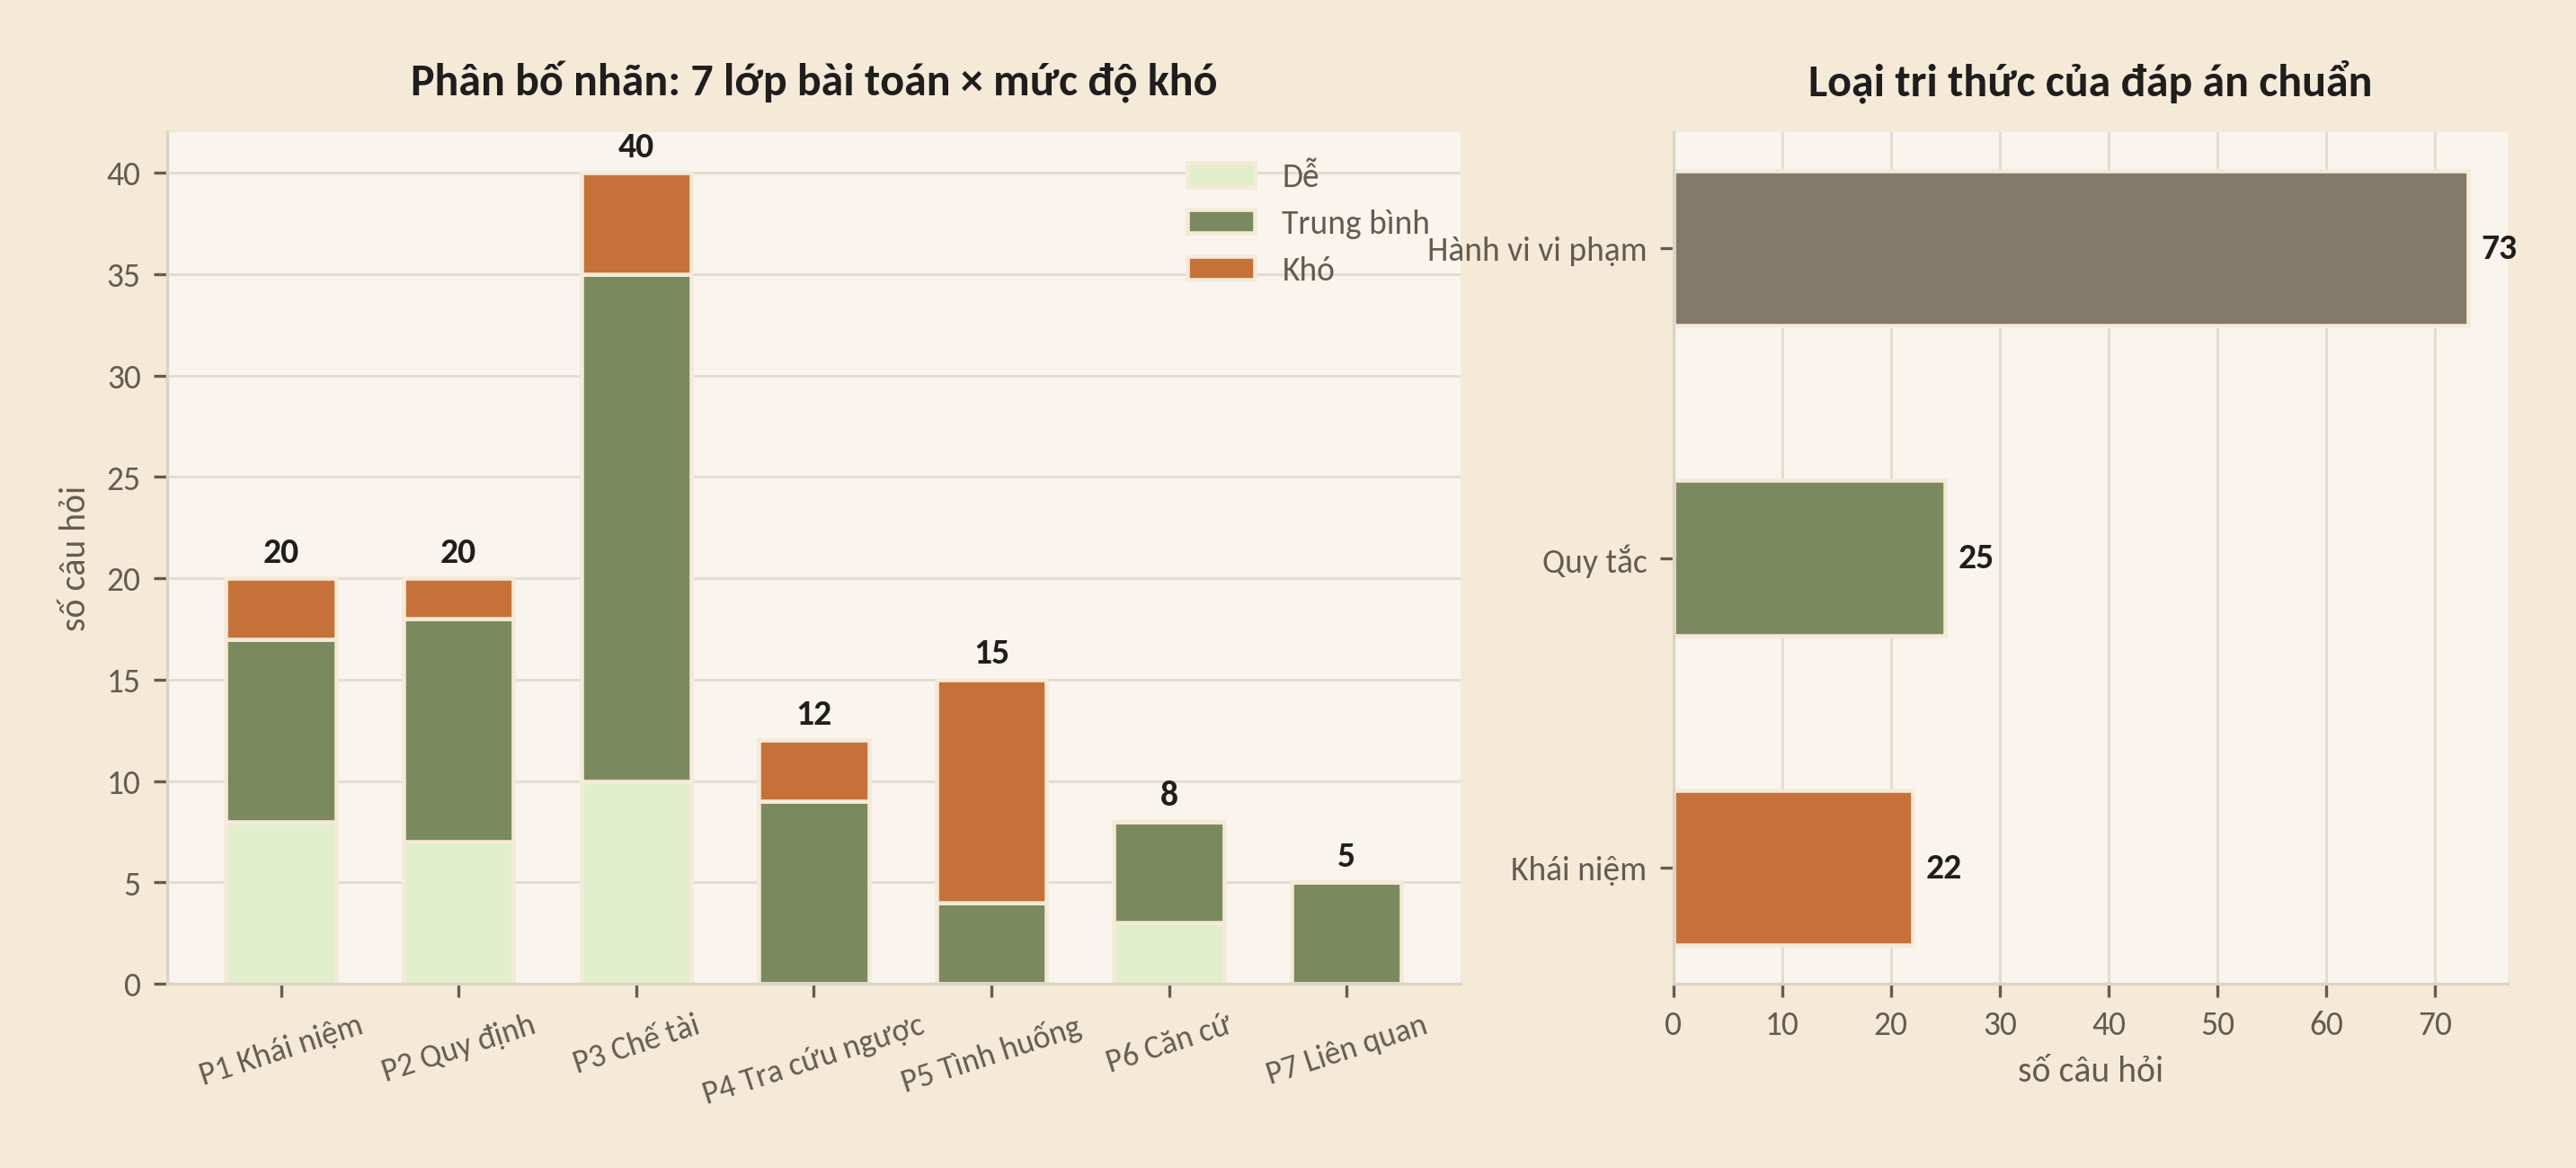
\includegraphics[width=\textwidth]{figures/hinh4_phan_bo_nhan.png}
\caption{Phân bố nhãn của bộ câu hỏi có đáp án chuẩn}
\label{fig:nhan}
\end{figure}

\subsubsection{Phân bố chủ đề}

Cơ sở tri thức chia thành 6 lĩnh vực và 55 nhóm hành vi. Tỉ trọng trong cơ sở tri thức và
trong bộ câu hỏi \emph{không} trùng nhau, và đây là chủ ý: lĩnh vực ``An toàn của người tham
gia giao thông'' chiếm 19\% cơ sở tri thức nhưng 43\% bộ câu hỏi, vì nồng độ cồn và mũ bảo
hiểm là hai chủ đề được hỏi nhiều nhất ngoài đời. Ngược lại, ``Điều kiện của phương tiện''
chiếm 17\% cơ sở tri thức nhưng chỉ 8\% bộ câu hỏi.

\begin{warnbox}
Nhóm ghi nhận đây là một \textbf{hạn chế của bộ đánh giá} chứ không giấu đi: bộ câu hỏi phản
ánh nhu cầu tra cứu phổ biến, nên chưa phủ đều mọi ngóc ngách của cơ sở tri thức --- tính
theo định danh, 120 câu mới chạm tới 115/527 mục tri thức truy hồi được (21,8\%). Một bộ đánh
giá phủ đều hơn là việc cần làm tiếp, nêu ở mục~\ref{sec:huong-phat-trien}.
\end{warnbox}

\begin{figure}[H]
\centering
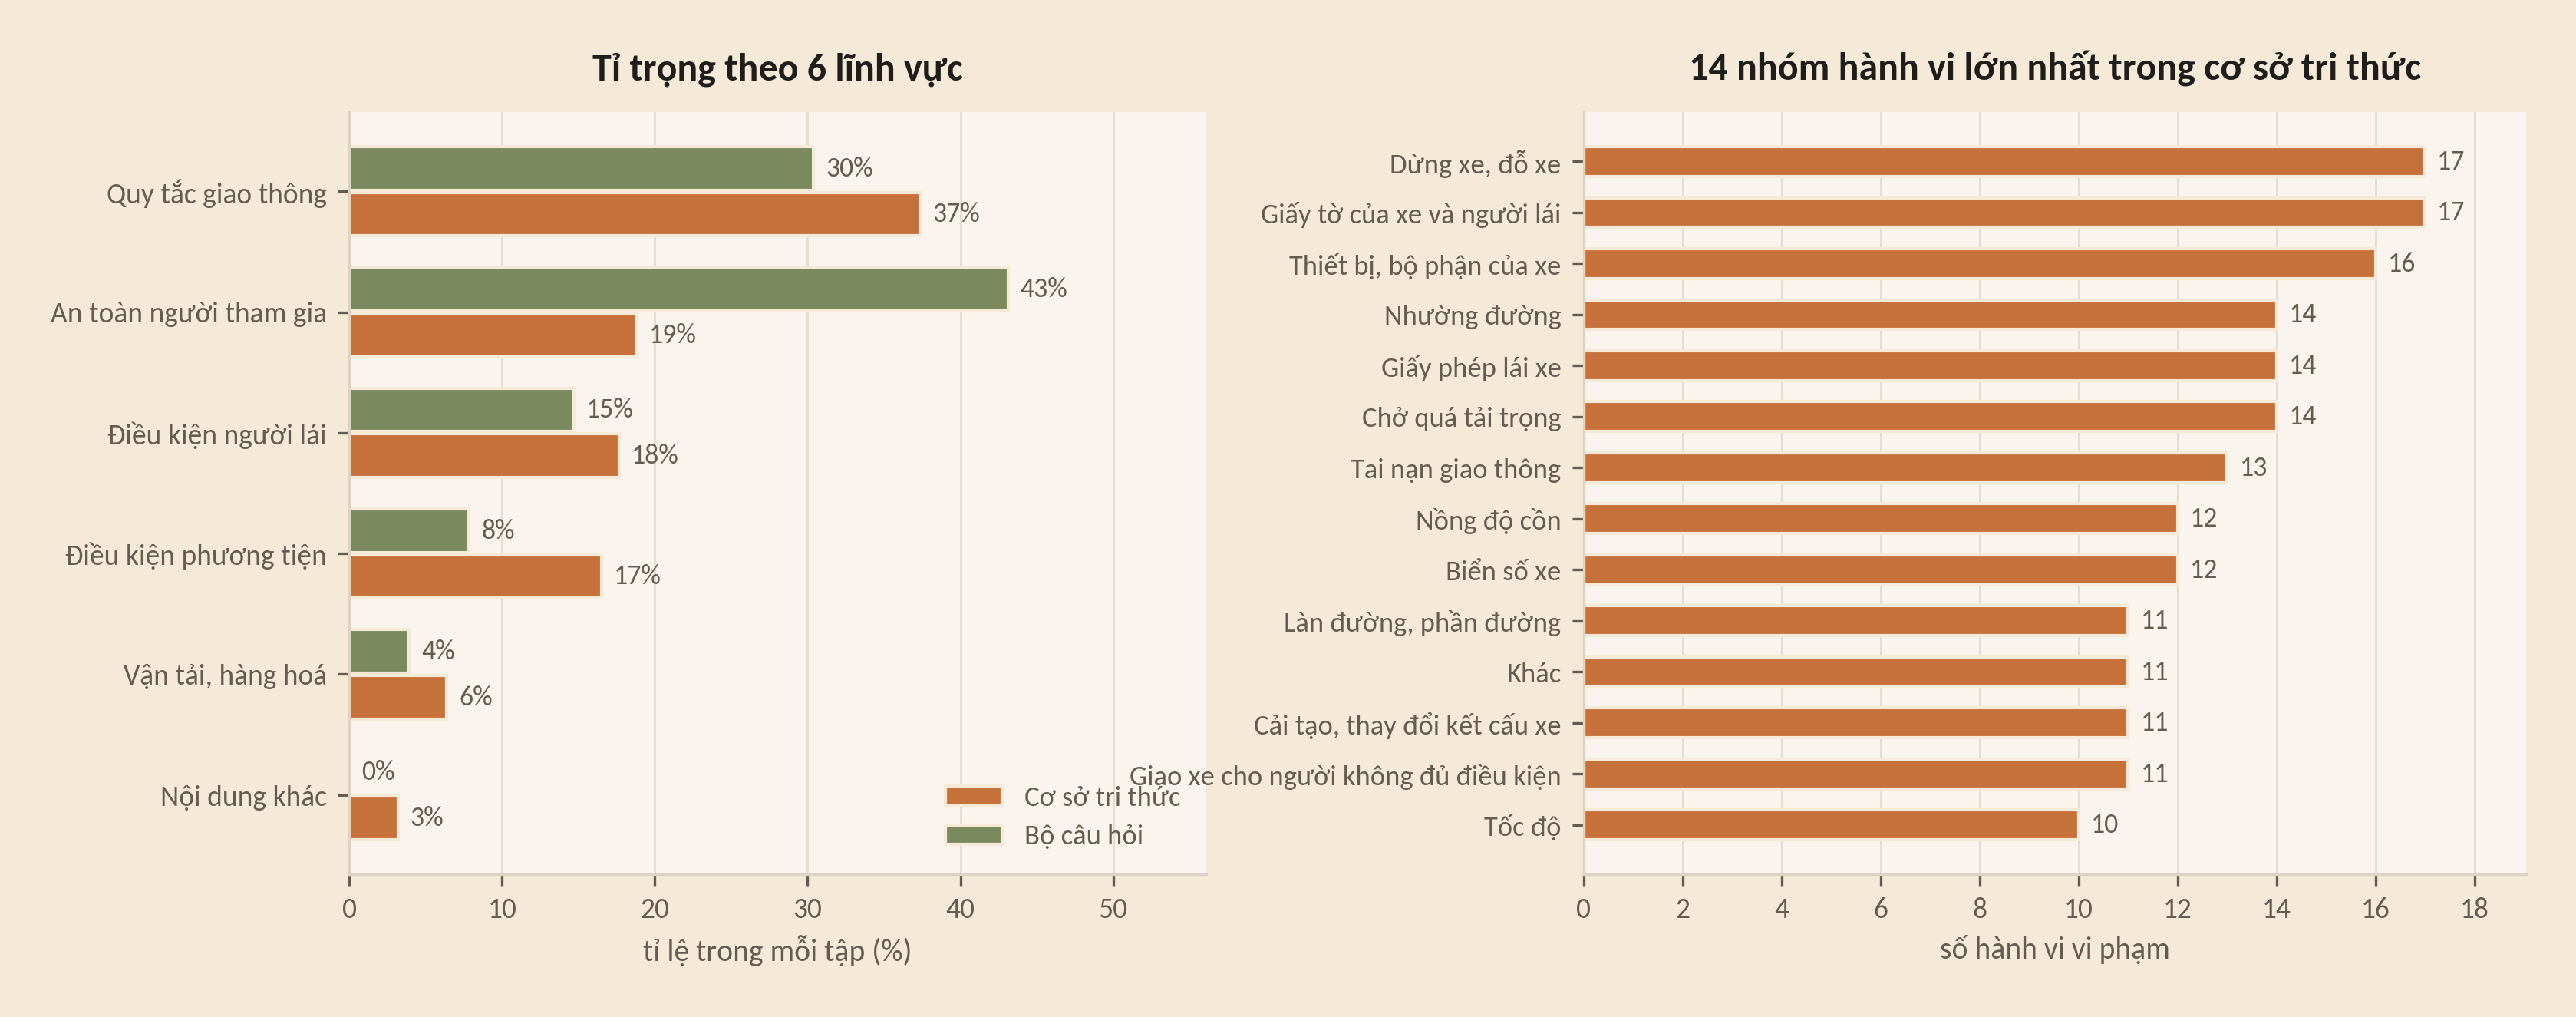
\includegraphics[width=\textwidth]{figures/hinh5_phan_bo_chu_de.png}
\caption{Phân bố chủ đề --- tỉ trọng lĩnh vực và nhóm hành vi}
\label{fig:chu-de}
\end{figure}

% ============================================================================
%  4. PHƯƠNG PHÁP VÀ THỰC NGHIỆM
% ============================================================================
\section{Phương pháp và thực nghiệm}
\label{sec:phuong-phap}

\subsection{Kiến trúc tổng thể}

Hệ thống gồm ba tầng nối tiếp (Hình~\ref{fig:kien-truc}). \code{QueryAnalyzer} biến câu hỏi
tiếng Việt thành một biểu diễn hình thức $Q$; \code{InferenceEngine} dùng $Q$ để chọn bộ giải
và truy hồi tri thức từ \code{IndexedKnowledgeBase}; hàm sinh văn bản ghép câu trả lời kèm
căn cứ pháp lý. Tầng dense embedding là tuỳ chọn và mặc định không được gọi --- lý do trình
bày ở mục~\ref{sec:han-che}.

\begin{figure}[H]
\centering
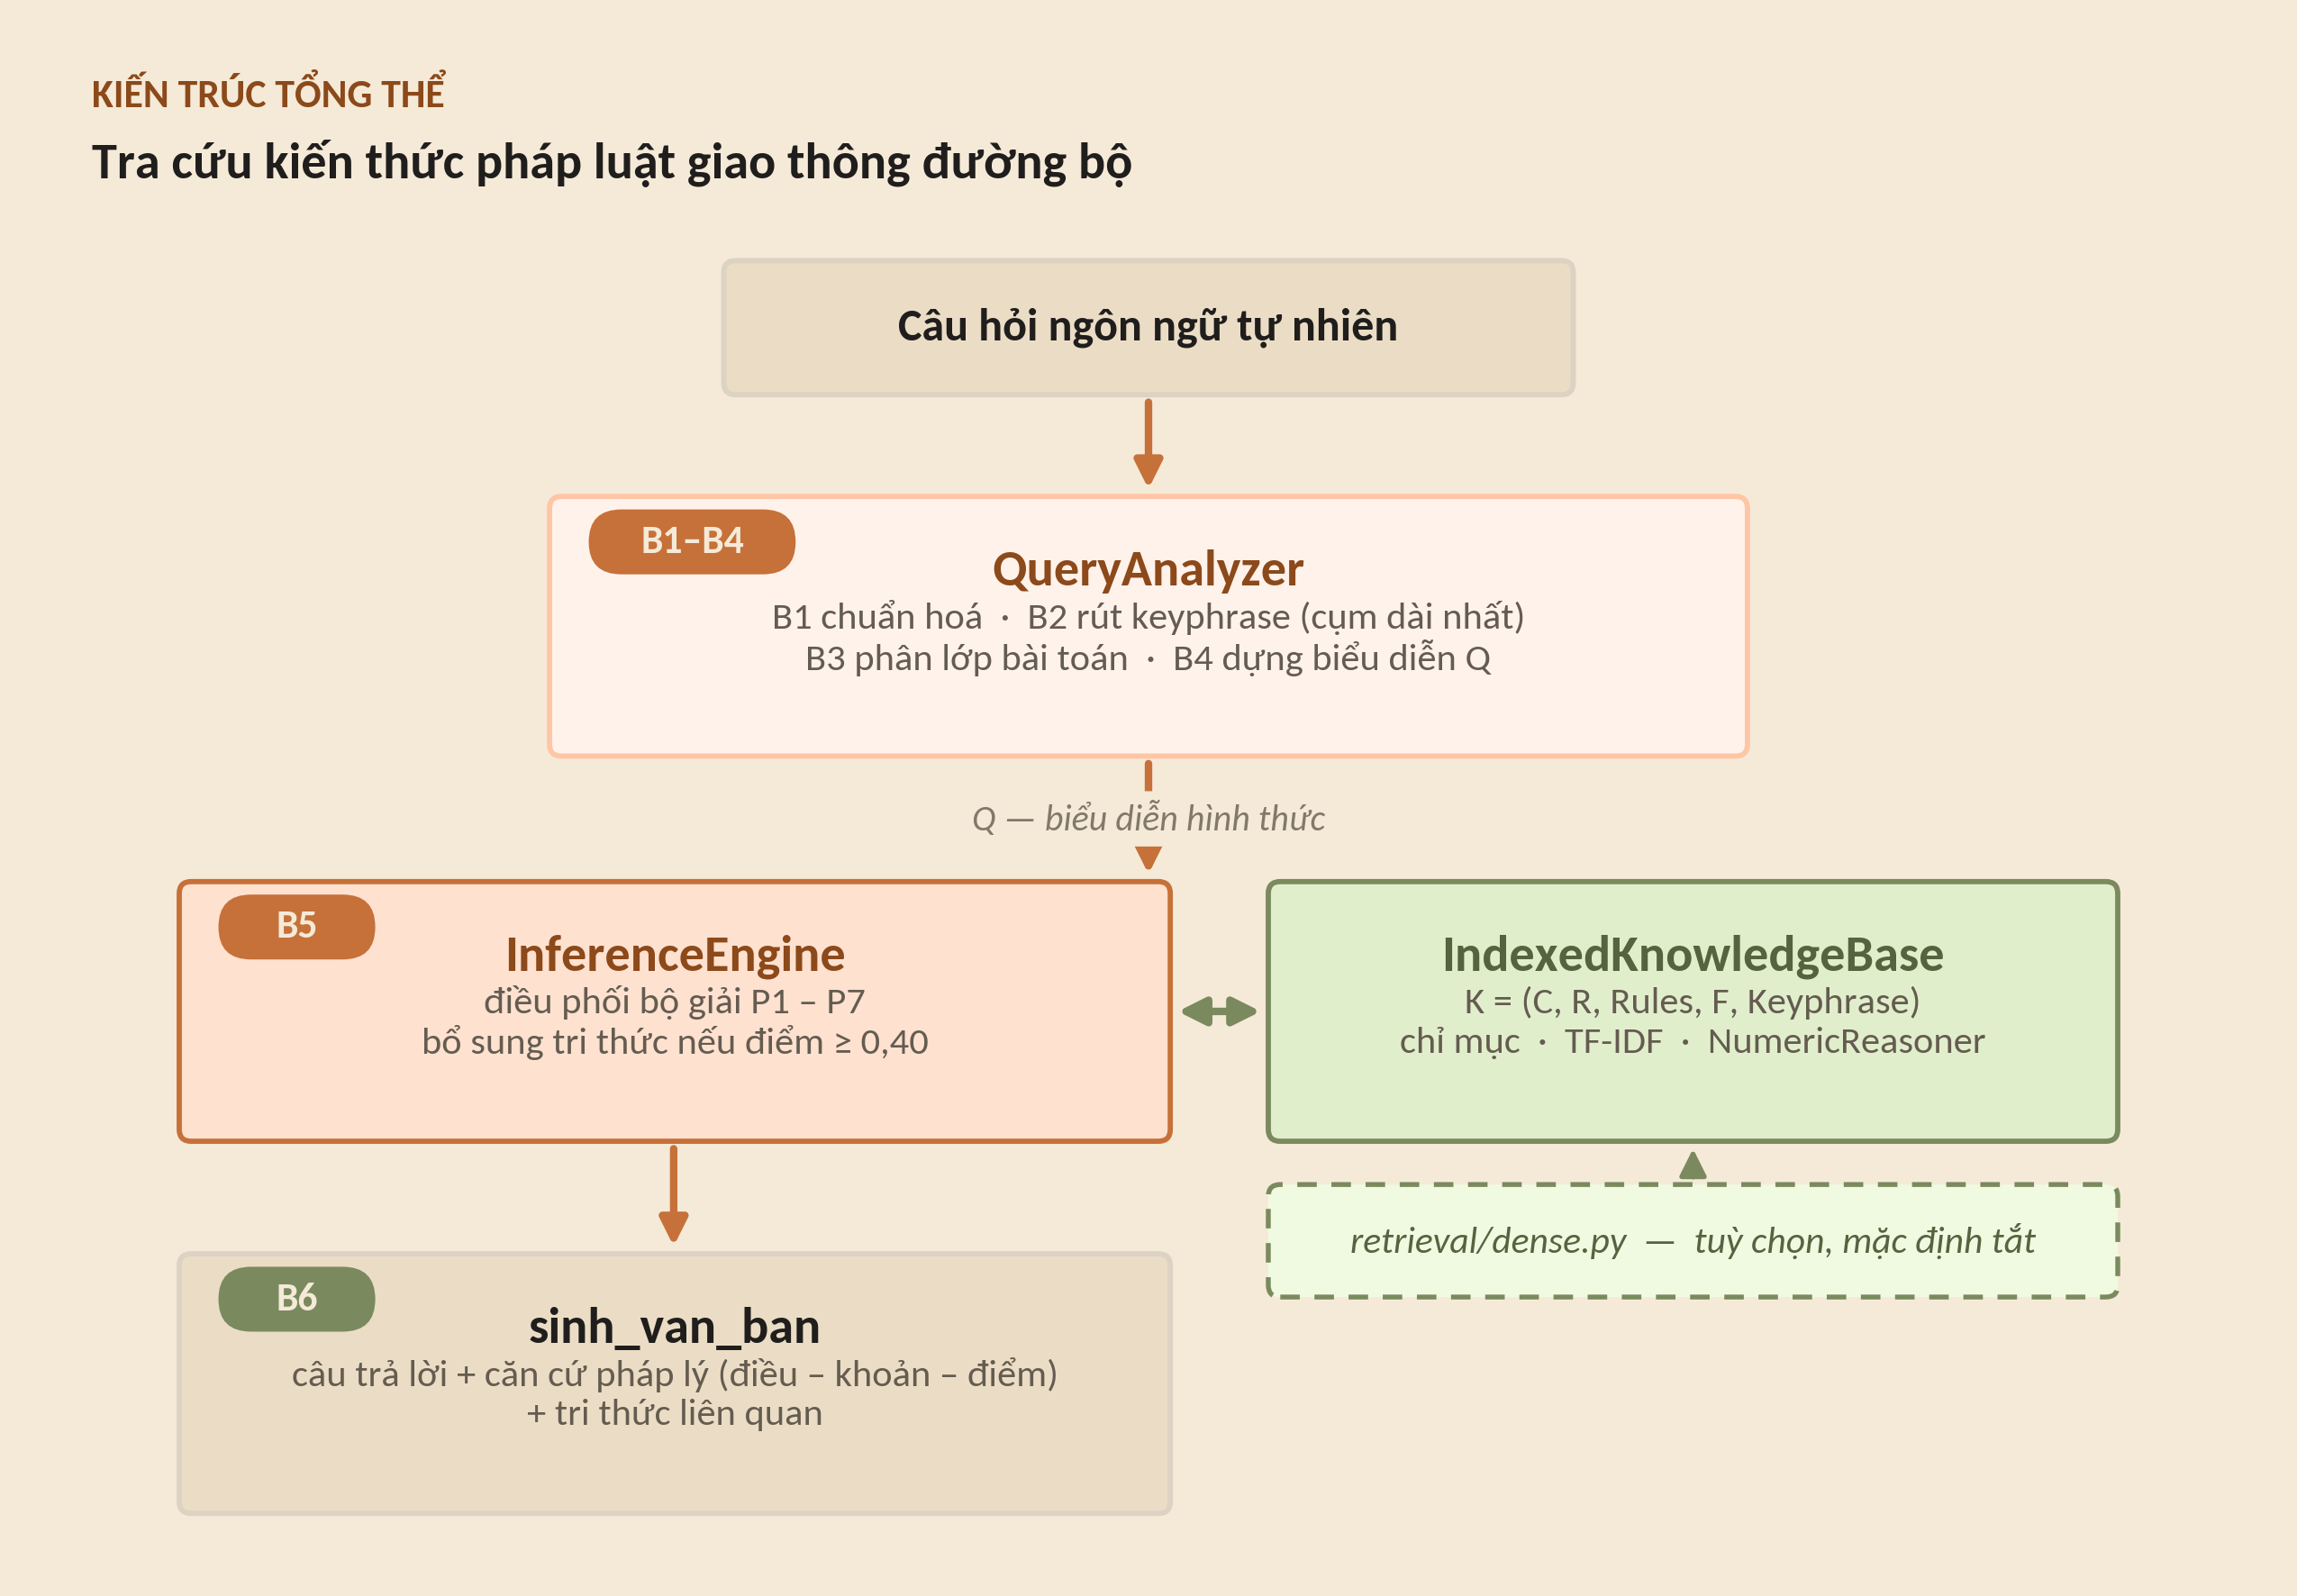
\includegraphics[width=0.96\textwidth]{figures/hinh1_kien_truc.png}
\caption{Kiến trúc hệ thống}
\label{fig:kien-truc}
\end{figure}

\subsection{Thuật giải xử lý truy vấn B1 -- B6}

\begin{table}[H]
\centering
\caption{Sáu bước xử lý một truy vấn}
\label{tab:b1-b6}
\renewcommand{\arraystretch}{1.2}
\begin{tabularx}{\textwidth}{@{}c >{\raggedright\arraybackslash}p{4.4cm} L@{}}
\toprule
\textbf{Bước} & \textbf{Việc} & \textbf{Hiện thực} \\
\midrule
B1 & Chuẩn hoá truy vấn         & Hạ chữ thường, chuẩn hoá Unicode, sinh bản không dấu \\
B2 & Rút trích keyphrase        & So khớp cụm dài nhất trên bản không dấu, không chồng lấn \\
B3 & Phân loại lớp bài toán     & Hàm điểm có trọng số trên sáu nhóm mẫu biểu thức chính quy \\
B4 & Dựng biểu diễn hình thức $Q$ & Keyphrase, nhóm, phương tiện, chủ thể, căn cứ, ràng buộc số \\
B5 & Suy diễn và truy hồi       & Bộ giải riêng cho từng lớp P1 -- P7 \\
B6 & Sinh câu trả lời           & Ghép nguyên văn điều khoản kèm căn cứ và tri thức liên quan \\
\bottomrule
\end{tabularx}
\end{table}

Thuật giải~\ref{alg:b1b6} mô tả toàn bộ quy trình ở mức giả mã.

\begin{algorithm}[H]
\small
\caption{Xử lý một truy vấn tra cứu pháp luật}
\label{alg:b1b6}
\KwIn{truy vấn $q$; mốc thời gian $t$; số kết quả $k$; cơ sở tri thức $K$}
\KwOut{$A(q,t) = (p, T, E)$}
$\hat q \leftarrow \mathrm{chuẩn\_hoá}(q)$;\quad $\bar q \leftarrow \mathrm{bỏ\_dấu}(\hat q)$ \tcp*{B1}
$KP \leftarrow \emptyset$;\quad $i \leftarrow 0$ \tcp*{B2: khớp cụm dài nhất}
\While{$i < |\bar q|$}{
  tìm $w \le 8$ lớn nhất sao cho cụm $\bar q[i..i{+}w)$ có trong từ điển $\mathit{Keyphrase}$\;
  \eIf{tìm thấy}{thêm cụm vào $KP$;\quad $i \leftarrow i + w$}{$i \leftarrow i + 1$}
}
$cc \leftarrow \mathrm{nhận\_dạng\_căn\_cứ}(\hat q)$;\quad $rb \leftarrow \mathrm{nhận\_dạng\_ràng\_buộc\_số}(\hat q)$\;
\eIf(\tcp*[f]{B3}){$cc \neq \emptyset$}{$p \leftarrow P6$}{$p \leftarrow \arg\max_{P}\ \mathrm{điểm\_lớp}(P \mid \bar q, KP, rb)$}
$Q \leftarrow (KP, \text{nhóm}, \text{phương tiện}, \text{chủ thể}, cc, rb)$ \tcp*{B4}
$T \leftarrow \mathrm{bộ\_giải}_p(Q, K)$, chỉ giữ $x$ có $t \in hl(x)$ \tcp*{B5}
\ForEach{loại tri thức còn thiếu trong $T$}{
  bổ sung các $x$ có $\mathrm{score}(x, q) \ge 0{,}40$\;
}
$E \leftarrow \{(\text{nguyên văn}(x), cc(x)) : x \in T\}$ \tcp*{B6}
\Return $(p,\ T[1..k],\ E)$\;
\end{algorithm}

Vì sao B2 phải khớp \emph{cụm dài nhất}: cụm ``nồng độ cồn'' phải thắng hai cụm rời ``nồng
độ'' và ``cồn''. Nếu khớp cụm ngắn trước, truy vấn sẽ trỏ sang mảng tri thức khác và mọi bước
sau đều sai theo.

\begin{figure}[H]
\centering
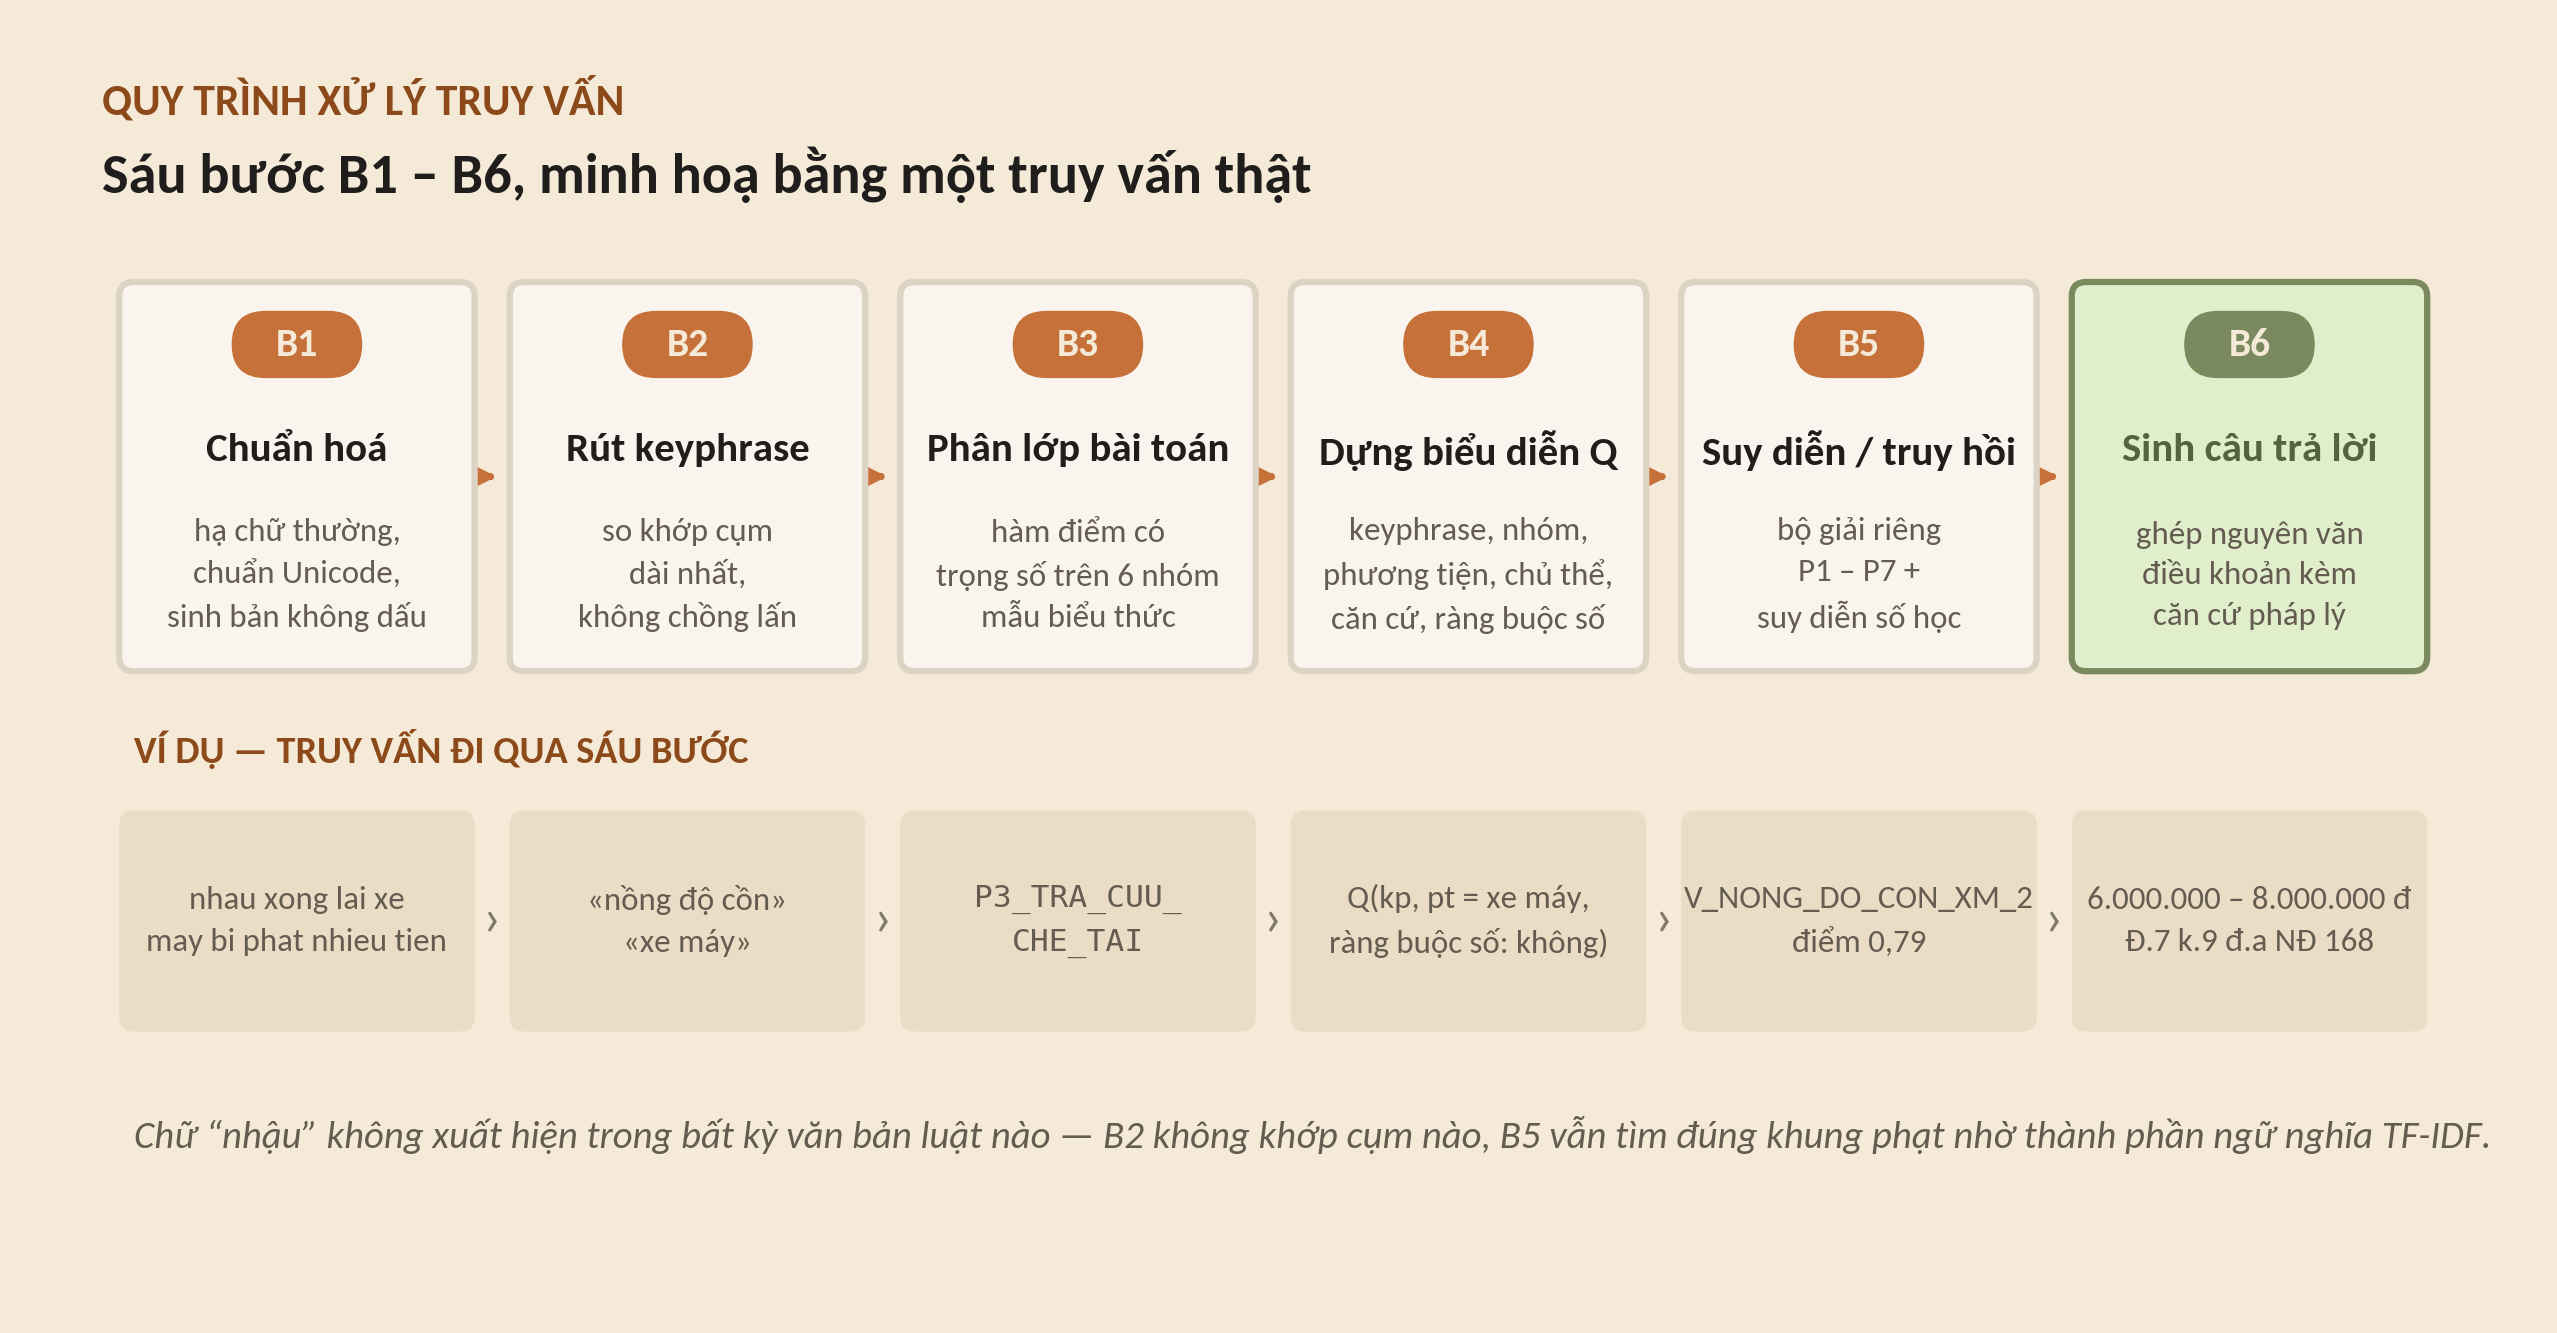
\includegraphics[width=0.9\textwidth]{figures/hinh2_luong_b1_b6.png}
\caption{Luồng xử lý truy vấn B1 -- B6 với một truy vấn thật}
\label{fig:luong}
\end{figure}

\subsection{Bảy lớp bài toán và bộ giải tương ứng}

\begin{table}[H]
\centering
\caption{Bảy lớp bài toán và câu hỏi tiêu biểu}
\label{tab:lop}
\renewcommand{\arraystretch}{1.2}
\begin{tabularx}{\textwidth}{@{}c >{\raggedright\arraybackslash}p{5.6cm} L@{}}
\toprule
\textbf{Lớp} & \textbf{Tên} & \textbf{Câu hỏi tiêu biểu} \\
\midrule
P1 & Tra cứu khái niệm, định nghĩa           & Xe cơ giới là gì? \\
P2 & Tra cứu quy định, quy tắc               & Quy tắc nhường đường tại nơi đường giao nhau? \\
P3 & Tra cứu chế tài                         & Vượt đèn đỏ xe máy phạt bao nhiêu? \\
P4 & Tra cứu ngược theo mức phạt / điểm trừ  & Lỗi nào bị trừ 10 điểm giấy phép lái xe? \\
P5 & Suy diễn tình huống nhiều hành vi       & Vừa vượt đèn đỏ vừa không có bằng thì tổng bao nhiêu? \\
P6 & Tra cứu theo căn cứ pháp lý             & Điều 6 khoản 9 điểm a NĐ 168/2024 nói về lỗi gì? \\
P7 & Tra cứu kiến thức liên quan             & Cho tôi thông tin về điểm giấy phép lái xe. \\
\bottomrule
\end{tabularx}
\end{table}

Điểm thiết kế đáng chú ý: \textbf{phân lớp không chặn kết quả}. Sau khi bộ giải của lớp được
chọn chạy xong, hệ thống vẫn bổ sung đủ ba loại tri thức (khái niệm, quy tắc, chế tài) nếu
còn thiếu và điểm vượt ngưỡng 0,40. Nhờ vậy một câu bị phân lớp sai vẫn có cơ hội trả đúng
--- đây chính là lý do Top-5 (95,00\%) cao hơn hẳn Top-1 (76,67\%).

\subsection{Hàm điểm lai}

Mỗi ứng viên tri thức $x$ được chấm theo
\begin{equation}
  \mathrm{score}(x, q) = \alpha \cdot s_{\text{keyphrase}}(x,q)
                       + \beta  \cdot s_{\text{ngữ nghĩa}}(x,q)
                       + \gamma \cdot s_{\text{ngữ cảnh}}(x,q)
  \label{eq:score}
\end{equation}
với $\alpha = 0{,}55$, $\beta = 0{,}30$, $\gamma = 0{,}15$.

\begin{table}[H]
\centering
\caption{Ba thành phần của hàm điểm và lý do chọn trọng số}
\label{tab:score}
\renewcommand{\arraystretch}{1.25}
\begin{tabularx}{\textwidth}{@{}>{\raggedright\arraybackslash}p{2.6cm} >{\raggedright\arraybackslash}p{5.0cm} L@{}}
\toprule
\textbf{Thành phần} & \textbf{Ý nghĩa} & \textbf{Vì sao trọng số đó} \\
\midrule
$s_{\text{keyphrase}}$ & Keyphrase trỏ thẳng tới định danh tri thức & Cao nhất (0,55) vì đây là tín hiệu chắc chắn: khớp đúng cụm từ pháp lý thì gần như không sai. \\
$s_{\text{ngữ nghĩa}}$ & Cosine TF-IDF char 3--5 gram kết hợp word 1--3 gram & 0,30 --- cứu các câu khẩu ngữ không có keyphrase, nhưng nhiễu hơn nên không được vượt keyphrase. \\
$s_{\text{ngữ cảnh}}$ & Khớp phương tiện, chủ thể, nhóm hành vi & 0,15 --- chỉ dùng để phân biệt các hành vi gần giống nhau, không đủ sức tự chọn kết quả. \\
\bottomrule
\end{tabularx}
\end{table}

Char $n$-gram chịu được lỗi chính tả và cách tách từ tiếng Việt; word $n$-gram giữ được cụm
nhiều từ. Với khái niệm và quy tắc, điểm ngữ nghĩa còn được trộn thêm 0,4 phần khớp riêng với
tên của mục tri thức: $s = 0{,}6\, s_{\text{nội dung}} + 0{,}4\, s_{\text{tên}}$.

\subsection{Suy diễn số học và hiệu lực theo thời gian}

Nhiều điều khoản phân khung theo ngưỡng số: nồng độ cồn chia ba mức, vượt tốc độ chia bốn
mức. So khớp từ khoá tìm ra đủ các khung nhưng không biết chọn khung nào.
\code{NumericReasoner} rút ngưỡng từ chính nguyên văn điều khoản thành một khoảng
$(a, b]$, so với giá trị $v$ trích từ câu hỏi và đẩy khung thoả $a < v \le b$ lên đầu.

\begin{keybox}
\textbf{Ví dụ.} \emph{``xe máy nồng độ cồn 0,3 mg/l phạt bao nhiêu''} $\Rightarrow$ $0{,}3$ thuộc
khung ``vượt quá 0,25 đến 0,4 miligam/1 lít khí thở'', không phải khung 0,25 hay khung trên
0,4. Hỏi liên tiếp 0,2 -- 0,3 -- 0,5 cho ba khung phạt khác nhau.
\end{keybox}

Về hiệu lực thời gian, mỗi mục tri thức mang khoảng $hl(x) = [\text{từ}, \text{đến})$ và mọi
truy vấn đều được lọc theo mốc $t$. Ví dụ quy tắc R15 về chở trẻ em dưới 10 tuổi mang nguyên
văn sau sửa đổi nên có hiệu lực từ 01/7/2026 theo Luật 118/2025, không phải 01/01/2025. Người
dùng đổi tham số \code{ngay=YYYY-MM-DD} là xem được cơ sở tri thức tại thời điểm đó.

\subsection{Cấu hình siêu tham số}

Toàn bộ siêu tham số được khai báo tường minh trong mã nguồn (hai tệp \code{engine.py} và \code{dense.py} nằm trong
thư mục \code{src/traffic\_law/}) và khoá lại bằng kiểm thử, không
có giá trị nào chỉnh ngầm lúc chạy.

\begin{table}[H]
\centering
\caption{Cấu hình siêu tham số của hệ thống}
\label{tab:sieu-tham-so}
\small
\renewcommand{\arraystretch}{1.2}
\begin{tabularx}{\textwidth}{@{}>{\raggedright\arraybackslash}p{3.5cm} >{\raggedright\arraybackslash}p{3.7cm} >{\raggedright\arraybackslash}p{2.1cm} L@{}}
\toprule
\textbf{Tham số} & \textbf{Giá trị} & \textbf{Vị trí} & \textbf{Ý nghĩa} \\
\midrule
ALPHA ($\alpha$) & 0,55 & \code{engine.py} & Trọng số làn keyphrase \\
BETA ($\beta$)   & 0,30 & \code{engine.py} & Trọng số làn ngữ nghĩa TF-IDF \\
GAMMA ($\gamma$) & 0,15 & \code{engine.py} & Trọng số làn ngữ cảnh \\
$k$ (top-$k$)    & 5    & tham số truy vấn           & Số kết quả trả về cho mỗi truy vấn \\
SUPPLEMENT\_\allowbreak THRESHOLD & 0,40 & \code{engine.py} & Ngưỡng bổ sung tri thức loại còn thiếu \\
Ngưỡng nhóm ngữ nghĩa & 0,24 · tối đa 2 nhóm & \code{engine.py} & Chặn suy đoán nhóm hành vi khi tín hiệu yếu \\
TF-IDF ký tự & \code{char\_wb}, $n$-gram 3--5, \code{sublinear\_tf} & \code{engine.py} & Chịu lỗi chính tả và cách tách từ \\
TF-IDF từ & \code{word}, $n$-gram 1--3, \code{sublinear\_tf} & \code{engine.py} & Giữ được cụm nhiều từ \\
Ngưỡng miền an toàn & 0,45 & \code{dense.py} & Giá trị lớn nhất còn giữ được cam kết không từ chối oan \\
Ngưỡng miền nghiêm ngặt & 0,52 & \code{dense.py} & Loại hết truy vấn rác nhưng từ chối oan --- không dùng mặc định \\
Mô hình dense (tuỳ chọn) & \code{paraphrase-}\newline\code{multilingual-}\newline\code{MiniLM-L12-v2} & \code{dense.py} & Chỉ bật khi cài gói tuỳ chọn, $\sim$470~MB \\
\bottomrule
\end{tabularx}
\end{table}

Hệ thống \textbf{không huấn luyện mô hình nào}: không có bước học tham số và không có tập huấn
luyện. Tuy vậy, cần nói rõ một điểm để không diễn giải quá số liệu: ba trọng số $\alpha, \beta,
\gamma$ được \emph{chọn và biện minh} bằng thí nghiệm loại bỏ thành phần
(mục~\ref{sec:ablation}) chạy trên \emph{chính} bộ 120 câu hỏi đánh giá. Bộ câu hỏi vì vậy vừa
là thước đo vừa là căn cứ để chọn cấu hình, và chưa có tập câu hỏi giữ lại (held-out) nào để
đo khả năng khái quát sang câu hỏi mới --- hạn chế này được ghi ở mục~\ref{sec:han-che}.

\subsection{Thiết lập thực nghiệm và chỉ số đo}
\label{sec:chi-so}

Bộ dữ liệu đánh giá gồm $N = 120$ câu hỏi; câu thứ $i$ có tập định danh đáp án chuẩn $G_i$,
lớp bài toán đúng và mức độ khó. Hệ thống trả về danh sách xếp hạng $T_i$ với $k = 5$ (riêng
lớp P4, P6 trả nguyên một tập thoả ràng buộc nên được chấm trên toàn tập). Ngoài ra có 40 truy
vấn ngoài lĩnh vực dùng để đo khả năng từ chối. Toàn bộ thực nghiệm chạy cục bộ, không gọi
dịch vụ ngoài.

Gọi $r_i$ là hạng của phần tử đúng đầu tiên trong $T_i$ ($r_i = \infty$ nếu không có). Các
chỉ số được tính như sau:
\begin{align}
  \text{Top-}n &= \frac{1}{N}\sum_{i=1}^{N} \mathbb{1}[\, r_i \le n \,],
  &
  \text{MRR} &= \frac{1}{N}\sum_{i=1}^{N} \frac{1}{r_i},
  \label{eq:topk-mrr}\\[2pt]
  P_i &= \frac{|G_i \cap T_i|}{|T_i|},\quad R_i = \frac{|G_i \cap T_i|}{|G_i|},
  &
  F1_i &= \frac{2 P_i R_i}{P_i + R_i},
  \label{eq:prf}
\end{align}
với precision, recall, F1 macro là trung bình của $P_i, R_i, F1_i$ trên $N$ câu. Khoảng tin cậy
95\% của một tỉ lệ $\hat p = x/n$ tính theo phương pháp Wilson:
\begin{equation}
  \frac{\hat p + \frac{z^2}{2n} \pm z\sqrt{\frac{\hat p(1-\hat p)}{n} + \frac{z^2}{4n^2}}}
       {1 + \frac{z^2}{n}}, \qquad z = 1{,}96.
  \label{eq:wilson}
\end{equation}
Để so hai cấu hình trên cùng bộ câu hỏi, dùng kiểm định McNemar chính xác: gọi $b$ là số câu
cấu hình mới đúng mà cấu hình cũ sai, $c$ là số câu ngược lại; khi đó
$p = \min\!\big(1,\ 2\sum_{j=0}^{\min(b,c)} \binom{b+c}{j} 2^{-(b+c)}\big)$.

\begin{table}[H]
\centering
\caption{Các chỉ số đo và ý nghĩa}
\label{tab:chi-so}
\renewcommand{\arraystretch}{1.2}
\begin{tabularx}{\textwidth}{@{}>{\raggedright\arraybackslash}p{4.3cm} L@{}}
\toprule
\textbf{Chỉ số} & \textbf{Đo điều gì} \\
\midrule
Độ chính xác phân lớp & Chất lượng bước B3 --- định tuyến tới đúng bộ giải \\
Top-1 / Top-3 / Top-5 & Chất lượng truy hồi ở các mức khoan dung khác nhau \\
MRR & Đáp án đúng thường nằm ở hạng nào \\
Precision / Recall / F1 (macro) & Độ sạch và độ phủ của tập trả về \\
Khoảng tin cậy 95\% (Wilson) & Độ bất định của mọi tỉ lệ do cỡ mẫu hữu hạn \\
Kiểm định McNemar & Chênh lệch giữa hai cấu hình có ý nghĩa thống kê hay không \\
AUC tách miền & Xác suất một câu hợp lệ được chấm cao hơn một truy vấn ngoài lĩnh vực \\
\bottomrule
\end{tabularx}
\end{table}

% ============================================================================
%  5. KẾT QUẢ VÀ PHÂN TÍCH
% ============================================================================
\section{Kết quả và phân tích}
\label{sec:ket-qua}

\subsection{Kết quả tổng thể}

\begin{table}[H]
\centering
\caption{Chỉ số đánh giá tổng thể trên 120 câu hỏi ($k = 5$), kèm khoảng tin cậy 95\% (Wilson)}
\label{tab:tong-the}
\renewcommand{\arraystretch}{1.2}
\begin{tabularx}{\textwidth}{@{}l r c L@{}}
\toprule
\textbf{Chỉ số} & \textbf{Giá trị} & \textbf{KTC 95\%} & \textbf{Ghi chú} \\
\midrule
Độ chính xác phân lớp & 95,83\% & [90,6\% -- 98,2\%] & 115/120 câu vào đúng lớp \\
\textbf{Top-1}        & \textbf{76,67\%} & [68,3\% -- 83,3\%] & Cổng chỉ số trong CI chặn mọi thay đổi làm tụt dưới mức này \\
Top-3                 & 90,83\% & [84,3\% -- 94,8\%] & 109/120 câu \\
Top-5                 & 95,00\% & [89,5\% -- 97,7\%] & 6/120 câu không có đáp án trong 5 kết quả \\
MRR                   & 0,8384  & ---                & Đáp án đúng thường nằm ở hạng 1--2 \\
Precision (macro)     & 0,3373  & ---                & Trần toán học 0,3707 --- xem mục~\ref{sec:kiem-dinh} \\
Recall (macro)        & 0,9306  & ---                & --- \\
F1 (macro)            & 0,4399  & ---                & --- \\
Thời gian trả lời TB  & 6,2~ms  & ---                & Chạy hoàn toàn cục bộ, đo trên máy cá nhân \\
\bottomrule
\end{tabularx}
\end{table}

Khoảng tin cậy được đưa vào có chủ đích. Với cỡ mẫu 120 câu, Top-1 76,67\% thực chất nằm
trong khoảng [68,3\% -- 83,3\%]. Nghĩa là một thay đổi làm Top-1 nhích 1--2 điểm phần trăm thì
\emph{không} kết luận được là cải tiến --- nhóm ghi rõ điều này để không diễn giải quá số liệu
mình có.

\subsection{Kết quả theo lớp bài toán}

\begin{table}[H]
\centering
\caption{Chỉ số theo từng lớp bài toán, kèm KTC 95\% của Top-1}
\label{tab:theo-lop}
\renewcommand{\arraystretch}{1.2}
\begin{tabularx}{\textwidth}{@{}L r r r c r@{}}
\toprule
\textbf{Lớp bài toán} & \textbf{$n$} & \textbf{Phân lớp} & \textbf{Top-1} & \textbf{KTC 95\% Top-1} & \textbf{Top-5} \\
\midrule
P1 · Tra cứu khái niệm     & 20 & 95,0\%  & 85,0\% & [64\% -- 95\%] & 95,0\% \\
\rowcolor{orange!8}
P2 · Tra cứu quy định      & 20 & 95,0\%  & 55,0\% & [34\% -- 74\%] & 85,0\% \\
P3 · Tra cứu chế tài       & 40 & 97,5\%  & 85,0\% & [71\% -- 93\%] & 97,5\% \\
P4 · Tra cứu ngược         & 12 & 100,0\% & 66,7\% & [39\% -- 86\%] & 100,0\% \\
P5 · Suy diễn tình huống   & 15 & 86,7\%  & 86,7\% & [62\% -- 96\%] & 93,3\% \\
P6 · Tra cứu căn cứ        & 8  & 100,0\% & 87,5\% & [53\% -- 98\%] & 100,0\% \\
P7 · Tra cứu liên quan     & 5  & 100,0\% & 40,0\% & [12\% -- 77\%] & 100,0\% \\
\bottomrule
\end{tabularx}
\end{table}

\textbf{Nhận xét.}
\begin{itemize}
  \item \textbf{P2} chỉ đạt Top-1 55,0\% nhưng Top-5 lên 85,0\%, và là lớp duy nhất có cả
        khoảng tin cậy nằm dưới mức chung 76,67\% --- tức là điểm yếu có thật chứ không do cỡ
        mẫu. Nguyên nhân: các quy tắc giao thông có nhiều điều khoản gần nghĩa; đáp án đúng
        thường \emph{có} trong danh sách trả về, chỉ chưa được xếp đầu.
  \item \textbf{P7} chỉ đạt Top-1 40,0\% nhưng Top-5 đạt 100,0\%. Với $n = 5$, con số 40\%
        thực chất là 2/5 câu và khoảng tin cậy rộng tới [12\% -- 77\%], nên gần như không kết
        luận được gì. Về bản chất, lớp ``tra cứu liên quan'' không có một đáp án duy nhất:
        người hỏi muốn một chùm tri thức, nên Top-5 mới là thước đo phù hợp.
  \item \textbf{P4} phân lớp đúng 100\% và Top-5 đạt 100\%, nhưng Top-1 chỉ 66,7\%: tra ngược
        theo mức phạt thường có nhiều hành vi cùng thoả điều kiện, và hệ thống trả về nguyên
        một \emph{tập} thoả ràng buộc, nên ``hạng 1'' ở lớp này là khái niệm ít ý nghĩa.
  \item \textbf{Câu nhiều đáp án chuẩn:} hệ lấy đủ toàn bộ đáp án ở 20/26 câu (76,92\%).
        Riêng lớp P4 đạt tuyệt đối; \textbf{P5 là nơi còn sót}: Top-5 tính là đúng chỉ cần
        tìm được \emph{một} vi phạm, nhưng muốn tính \emph{tổng} mức phạt thì phải tìm đủ
        mọi vi phạm --- điều này mới đạt 9/15 câu (60\%).
\end{itemize}

\subsection{Kiểm định ý nghĩa thống kê}
\label{sec:kiem-dinh}

Bốn kiểm định dưới đây trả lời bốn câu hỏi mà một bảng chỉ số đơn thuần không trả lời được.
Tất cả sinh ra từ \code{eval/kiem\_dinh.py}.

\subsubsection{Suy diễn số học có thật sự cải thiện, hay chỉ là may rủi?}

Kiểm định McNemar trên cùng bộ câu hỏi, so cấu hình C (lai ba thành phần) với cấu hình D
(thêm suy diễn số học): \textbf{12 câu} chuyển từ sai sang đúng, \textbf{0 câu} chuyển ngược
lại, $p = 0{,}000488$. Với $p < 0{,}001$, cải thiện này không phải ngẫu nhiên. Đáng chú ý hơn
cả trị số $p$ là hình dạng bảng chéo: không có câu nào bị suy diễn số học làm hỏng, nghĩa là
thành phần này chỉ thêm chứ không phá.

\subsubsection{Precision 0,3373 là kém hay đã kịch trần?}

Vì hệ trả $k = 5$ kết quả trong khi 94/120 câu chỉ có một mẩu tri thức đúng, precision của
những câu đó tối đa là $1/5 = 0{,}20$. Tính trần cho từng câu,
$P_i^{\max} = \min(|G_i|, |T_i|)/|T_i|$, rồi lấy trung bình được \textbf{0,3707}. Giá trị đo
được 0,3373 tương đương \textbf{91,0\%} của trần đó. Kết luận: precision thấp là hệ quả của
thiết kế top-$k$, không phải khiếm khuyết của mô hình --- và recall macro 0,9306 mới là chỉ số
phản ánh đúng mục tiêu của một hệ tra cứu.

\subsubsection{Hệ có chịu được truy vấn gõ không dấu?}

Chạy lại toàn bộ bộ câu hỏi sau khi bỏ dấu tiếng Việt: Top-1 76,67\%, Top-5 95,00\%, phân lớp
95,83\% --- \textbf{trùng khớp tuyệt đối} với bản có dấu ở cả bảy lớp bài toán. Có hai cơ chế
cùng bảo đảm điều này: (i) mọi keyphrase đều lưu kèm bản không dấu và B1 chuẩn hoá về bản đó;
(ii) hai bộ nhận dạng cấu trúc --- căn cứ điều khoản và ràng buộc số --- có bộ mẫu riêng cho
câu gõ không dấu.

\begin{warnbox}
Cơ chế (ii) là kết quả của chính phép kiểm định này. Ở phiên bản trước, bộ nhận dạng chỉ dò mẫu
có dấu nên khi bỏ dấu, lớp P6 rơi từ 7/8 xuống 0/8 và P4 từ 8/12 xuống 3/12 (Top-1 tổng còn
66,67\%). Lỗi đã được sửa và khoá bằng 24 test; bộ mẫu không dấu cố ý chặt hơn, vì mất dấu thì
``đèn'' và ``đến'', ``tự'' và ``từ'' trùng mặt chữ. Chỉ số trên câu có dấu không đổi một chữ số
nào sau khi sửa.
\end{warnbox}

\subsubsection{Mọi câu hỏi có thật sự chấm được?}

Có test kiểm chứng rằng toàn bộ 120/120 câu đều có đáp án chuẩn giải được về tri thức
\emph{có thật} trong cơ sở tri thức, không định danh treo nào. Nếu bước này không được kiểm,
mọi chỉ số ở trên đều vô nghĩa vì hệ thống có thể đang bị chấm trên những câu không thể đúng.

\subsection{Thí nghiệm loại bỏ thành phần}
\label{sec:ablation}

Để chứng minh từng thành phần của hàm điểm thực sự đóng góp chứ không phải chọn trọng số cảm
tính, nhóm chạy thí nghiệm loại bỏ thành phần trên cả 120 câu hỏi.

\begin{table}[H]
\centering
\caption{Kết quả loại bỏ thành phần (ablation) trên 120 câu hỏi}
\label{tab:ablation}
\renewcommand{\arraystretch}{1.2}
\begin{tabularx}{\textwidth}{@{}L r r r@{}}
\toprule
\textbf{Cấu hình} & \textbf{Top-1} & \textbf{Top-5} & \textbf{MRR} \\
\midrule
A. Chỉ so khớp ngữ nghĩa (TF-IDF)          & 58,3\% & 89,2\% & 0,7054 \\
B. Chỉ so khớp keyphrase                   & 35,8\% & 59,2\% & 0,4381 \\
C. Lai keyphrase + ngữ nghĩa + ngữ cảnh    & 66,7\% & 94,2\% & 0,7759 \\
\textbf{D. Hệ thống đầy đủ (C + suy diễn số học)} & \textbf{76,7\%} & \textbf{95,0\%} & \textbf{0,8384} \\
\bottomrule
\end{tabularx}
\end{table}

\begin{table}[H]
\centering
\caption{Ablation riêng trên 22 câu hỏi có giá trị số (nồng độ cồn, tốc độ)}
\label{tab:ablation-so}
\renewcommand{\arraystretch}{1.2}
\begin{tabularx}{\textwidth}{@{}L r r r@{}}
\toprule
\textbf{Cấu hình} & \textbf{Top-1} & \textbf{Top-5} & \textbf{MRR} \\
\midrule
C. Lai keyphrase + ngữ nghĩa + ngữ cảnh          & 40,9\% & 95,5\%  & 0,6364 \\
\textbf{D. Hệ thống đầy đủ (C + suy diễn số học)} & \textbf{95,5\%} & \textbf{100,0\%} & \textbf{0,9773} \\
\bottomrule
\end{tabularx}
\end{table}

\textbf{Nhận xét.}
\begin{itemize}
  \item Keyphrase đứng riêng (35,8\%) \emph{yếu hơn} TF-IDF đứng riêng (58,3\%), nhưng vẫn xứng
        đáng nhận trọng số cao nhất 0,55. Lý do: nó thua về \textbf{độ phủ} chứ không thua về
        \textbf{độ chính xác} --- câu nào có keyphrase thì gần như chắc đúng, chỉ là nhiều câu
        khẩu ngữ không có keyphrase nào.
  \item Lai ba thành phần đưa Top-1 lên 66,7\%: TF-IDF lo phần phủ, keyphrase lo phần chuẩn.
        Hai tín hiệu bù trừ nhau chứ không trùng lặp.
  \item Thêm suy diễn số học đưa Top-1 lên 76,7\%. Riêng 22 câu có giá trị số, Top-1 nhảy từ
        40,9\% lên 95,5\% trong khi Top-5 gần như không đổi. So khớp từ khoá \emph{vẫn tìm ra}
        đủ các khung phạt, nó chỉ không biết \emph{chọn khung nào}; suy diễn số học giải quyết
        đúng khâu đó, và cải thiện này có ý nghĩa thống kê ($p = 0{,}000488$).
  \item Lưu ý kỹ thuật: cấu hình C chỉ tắt \emph{bảng tra theo đại lượng} của bộ suy diễn số
        học, phần so ngưỡng vẫn chạy. Vì vậy mức tăng 10 điểm là \emph{cận dưới} của đóng góp
        thật.
\end{itemize}

\subsection{Phân tích lỗi sâu}

Thay vì chỉ liệt kê câu sai, nhóm chạy lại toàn bộ bộ câu hỏi, ghi \emph{hạng} của đáp án chuẩn
trong danh sách trả về, rồi quy mỗi ca chưa tối ưu về một nguyên nhân gốc duy nhất theo thứ tự
ưu tiên. Kết quả: \textbf{31/120 ca chưa tối ưu}. Trong đó chỉ 6 ca đáp án rơi hẳn ngoài
Top-5; 22 ca đáp án \emph{vẫn} nằm trong danh sách trả về nhưng không đứng đầu; 3 ca đáp án đã
ở hạng 1 nhưng câu hỏi bị gán sai lớp bài toán. Nói cách khác, phần lớn cái gọi là ``lỗi'' ở đây
là lỗi \textbf{xếp hạng}, không phải lỗi tìm kiếm.

\begin{table}[H]
\centering
\caption{Sáu nhóm nguyên nhân gốc và số ca}
\label{tab:nguyen-nhan}
\renewcommand{\arraystretch}{1.2}
\begin{tabularx}{\textwidth}{@{}c L r c@{}}
\toprule
\textbf{Mã} & \textbf{Nguyên nhân gốc} & \textbf{Số ca} & \textbf{Mức độ} \\
\midrule
L5 & Khoảng trống từ vựng làm tụt hạng        & 15 & Vừa \\
L1 & Định tuyến sai lớp bài toán              & 5  & Nặng \\
L3 & Thứ tự trong tập trả về (P4/P6/P7)       & 5  & Nhẹ \\
L2 & Trượt hẳn ngoài Top-$k$                  & 4  & Nặng \\
L4 & Câu nhiều đáp án chuẩn                   & 1  & Nhẹ \\
L6 & Khác                                     & 1  & Vừa \\
\midrule
   & \textbf{Tổng}                            & \textbf{31} & \\
\bottomrule
\end{tabularx}
\end{table}

\begin{figure}[H]
\centering
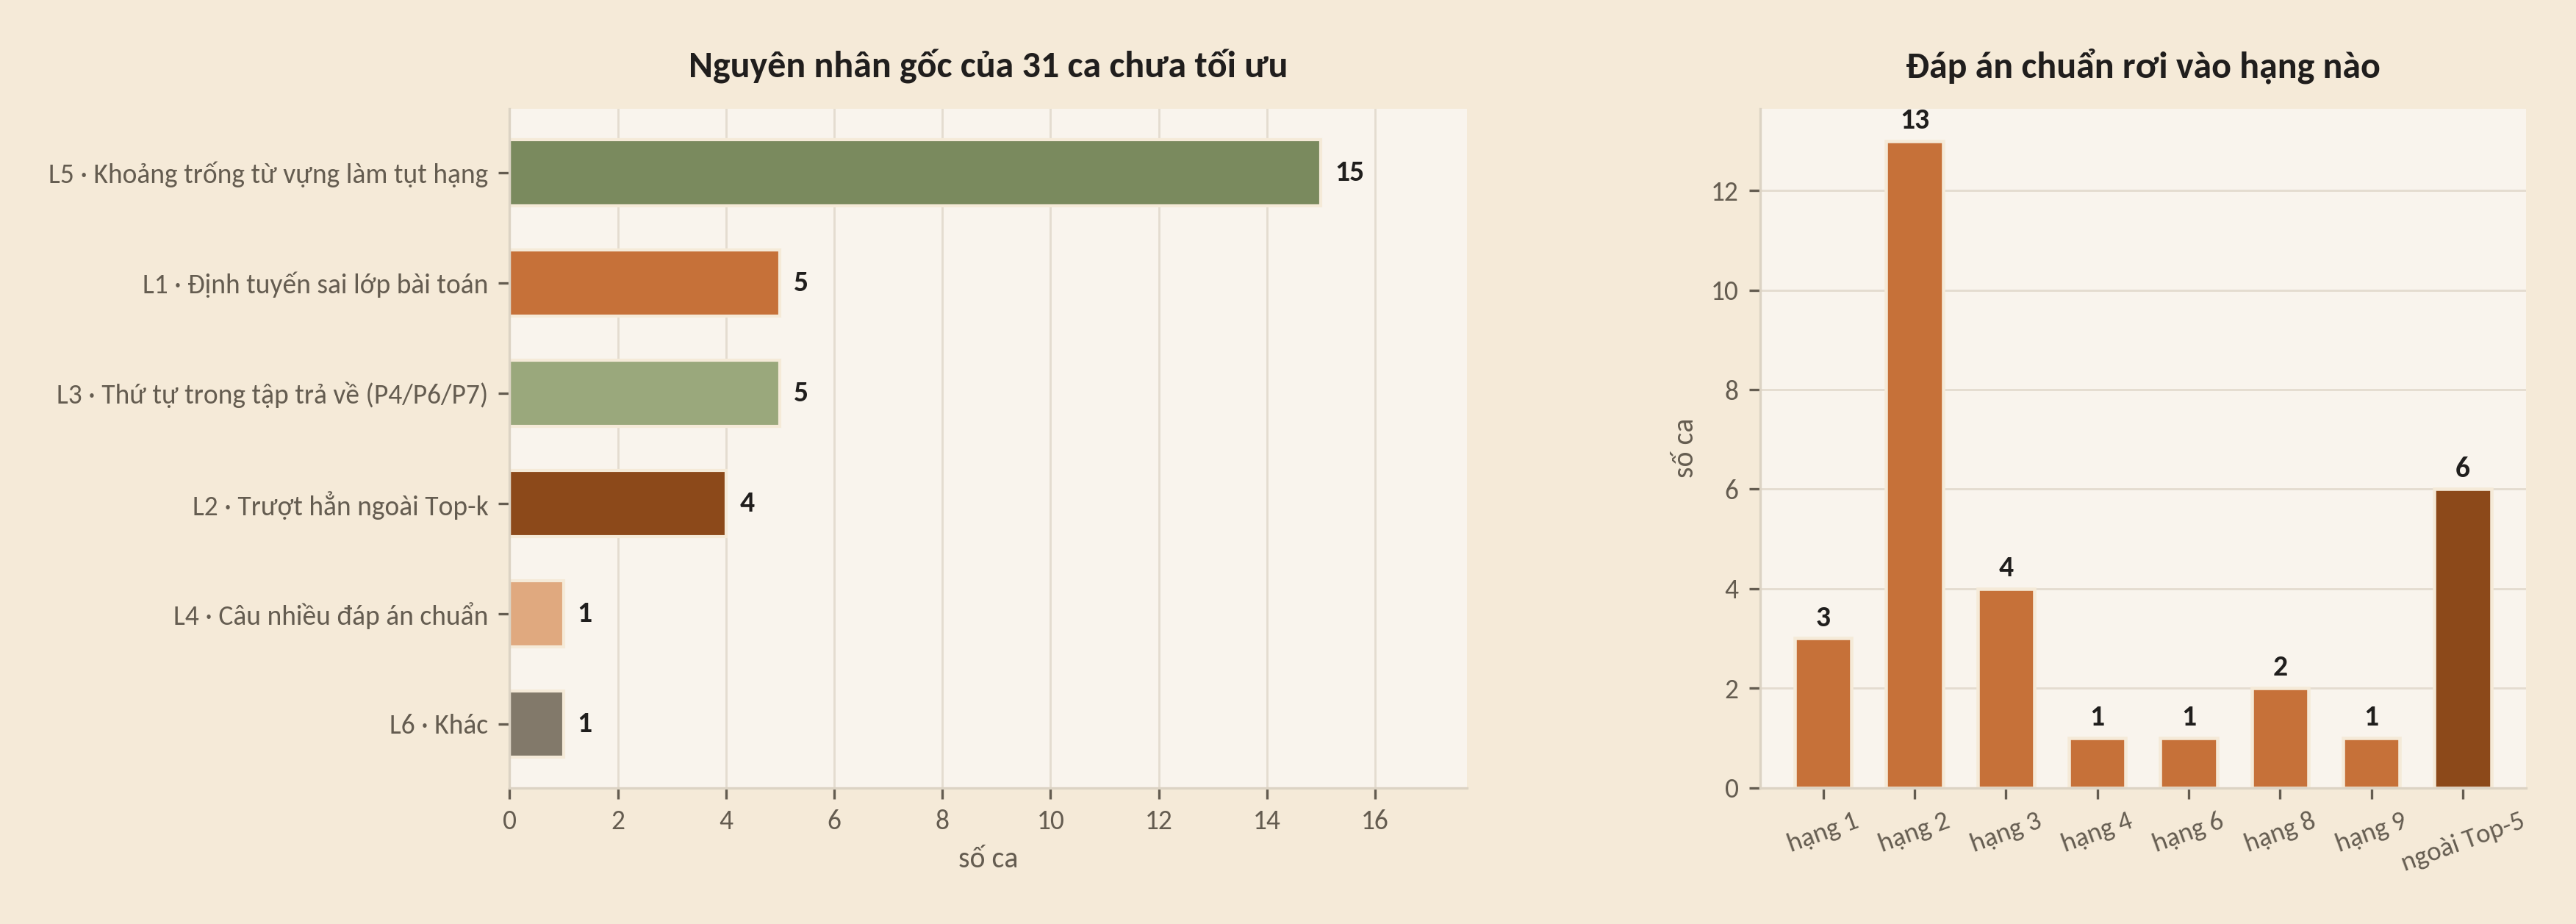
\includegraphics[width=\textwidth]{figures/hinh6_phan_tich_loi.png}
\caption{Phân tích lỗi sâu --- nguyên nhân gốc và hạng của đáp án chuẩn}
\label{fig:loi}
\end{figure}

\textbf{Diễn giải từng nhóm.}
\begin{itemize}
  \item \textbf{L5 --- Khoảng trống từ vựng} (15 ca, nhóm lớn nhất). Câu hỏi dùng từ đời thường
        không xuất hiện trong bất kỳ cụm từ khoá nào của đáp án: ``nón bảo hiểm'' thay vì ``mũ
        bảo hiểm'', ``bằng lái'' thay vì ``giấy phép lái xe''. Làn keyphrase im lặng, chỉ còn
        TF-IDF gánh, nên đáp án tụt xuống hạng 2--3 chứ hiếm khi rơi hẳn. Đây là lỗi sửa được
        bằng \emph{dữ liệu} (bổ sung biến thể khẩu ngữ), không cần đổi thuật giải.
  \item \textbf{L1 --- Định tuyến sai lớp} (5 ca, nặng nhất). Bước B3 chọn nhầm lớp nên bộ giải
        sai kiểu chạy. Ví dụ ``Đèn giao thông có mấy màu?'' bị đẩy sang P7 vì câu quá ngắn;
        ``Bằng lái bị trừ hết 12 điểm rồi thì sao\dots'' bị đẩy sang P4 vì con số 12 kích hoạt
        mẫu tra cứu ngược và nhận về danh sách rỗng.
  \item \textbf{L2 --- Trượt hẳn ngoài Top-5} (4 ca). Đây mới là lỗi người dùng thật sự cảm nhận
        được. Cả bốn ca đều là câu khẩu ngữ dài kể tình huống, hoặc câu dạng có/không (``Gặp đèn
        đỏ thì có được đi tiếp không?'') --- người hỏi chờ một câu khẳng định, hệ thống trả điều
        khoản gần nghĩa nhất.
  \item \textbf{L3 --- Thứ tự trong tập trả về} (5 ca, nhẹ nhất). Toàn bộ thuộc lớp P4/P6/P7,
        nơi hệ thống trả nguyên một tập thoả ràng buộc. Đáp án có trong tập, chỉ không đứng đầu
        --- đây là vấn đề trình bày chứ không phải truy hồi.
  \item \textbf{L4 và L6} (mỗi nhóm 1 ca). Hạng 1 là một mẩu tri thức cũng hợp lệ nhưng không
        trùng mẩu được chấm.
\end{itemize}

\begin{table}[H]
\centering
\caption{Một số ca tiêu biểu và nguyên nhân}
\label{tab:ca-tieu-bieu}
\small
\renewcommand{\arraystretch}{1.2}
\begin{tabularx}{\textwidth}{@{}c L c >{\raggedright\arraybackslash}p{4.3cm}@{}}
\toprule
\textbf{Mã} & \textbf{Câu hỏi} & \textbf{Hạng} & \textbf{Nguyên nhân} \\
\midrule
Q011 & Đèn giao thông có mấy màu? & 1 & L1 · Định tuyến sai lớp \\
Q020 & Mấy cái xe tự chạy không cần người lái ấy, trong luật gọi là gì\dots & ngoài Top-5 & L2 · Trượt ngoài Top-$k$ \\
Q021 & Gặp đèn đỏ thì có được đi tiếp không? & ngoài Top-5 & L2 · Trượt ngoài Top-$k$ \\
Q032 & Bằng lái bị trừ hết 12 điểm rồi thì sao, có được chạy xe nữa không\dots & ngoài Top-5 & L1 · Định tuyến sai lớp \\
Q035 & Chở con nhỏ trên ô tô thì luật quy định cháu ngồi ở đâu? & ngoài Top-5 & L2 · Trượt ngoài Top-$k$ \\
Q080 & Không chịu dừng xe khi cảnh sát giao thông ra hiệu kiểm tra thì\dots & ngoài Top-5 & L1 · Định tuyến sai lớp \\
Q096 & Nhóm em 4 đứa đi chung một xe máy, không ai đội mũ bảo hiểm\dots & 1 & L1 · Định tuyến sai lớp \\
Q101 & Xe ô tô của tôi bị che mất biển số và đã quá hạn đăng kiểm\dots & ngoài Top-5 & L2 · Trượt ngoài Top-$k$ \\
\bottomrule
\end{tabularx}
\end{table}

\subsection{Giải thích: vì sao các con số lại như vậy}

Bốn cơ chế dưới đây giải thích gần như toàn bộ hình dạng của kết quả.
\begin{enumerate}
  \item \textbf{Vì sao Top-5 (95,00\%) bỏ xa Top-1 (76,67\%)?} Vì cơ chế bổ sung tri thức không
        để bước phân lớp chặn kết quả: kể cả khi B3 chọn sai lớp, hệ vẫn nạp thêm tri thức của
        các loại còn thiếu nếu điểm vượt 0,40. Đáp án đúng hiếm khi biến mất khỏi danh sách,
        chỉ thường không đứng đầu --- đúng như 22 ca ở Bảng~\ref{tab:nguyen-nhan}.
  \item \textbf{Vì sao khoảng cách đó lớn nhất ở P2?} Quy tắc giao thông là loại tri thức có
        nhiều điều khoản gần nghĩa nhất --- nhường đường, chuyển hướng, quay đầu chia sẻ rất
        nhiều từ vựng. Cả ba làn điểm đều cho các ứng viên này số gần nhau, và hệ chưa có tín
        hiệu nào tách chúng ngoài độ tương đồng văn bản.
  \item \textbf{Vì sao suy diễn số học tạo khác biệt lớn (40,9\% $\to$ 95,5\%) mà Top-5 gần như
        không đổi?} Vì bài toán ở nhóm câu này không phải \emph{tìm} mà là \emph{chọn}. Các khung
        phạt của cùng một hành vi có văn bản gần như giống hệt nhau, chỉ khác con số ngưỡng; chỉ
        khi so sánh khoảng số mới chọn đúng được.
  \item \textbf{Vì sao hệ chưa từ chối được truy vấn ngoài lĩnh vực?} Vì đặc trưng TF-IDF mặc
        định không tách được hai phân bố: 56/120 câu hợp lệ chấm điểm thấp hơn hoặc bằng truy
        vấn rác, nên không tồn tại ngưỡng nào vừa loại hết rác vừa không từ chối oan
        (mục~\ref{sec:han-che}).
\end{enumerate}

\subsection{Kiểm thử nghiệm thu và kiểm thử tự động}

\begin{table}[H]
\centering
\caption{Mười hai ca nghiệm thu chức năng}
\label{tab:nghiem-thu}
\small
\renewcommand{\arraystretch}{1.18}
\begin{tabularx}{\textwidth}{@{}c >{\raggedright\arraybackslash}p{2.9cm} L c@{}}
\toprule
\textbf{Mã} & \textbf{Nhóm} & \textbf{Câu hỏi} & \textbf{Kết quả} \\
\midrule
TC01 & Lớp bài toán    & Xe cơ giới là gì? & \dat{} Đạt \\
TC02 & Lớp bài toán    & Người lái xe phải mang theo giấy tờ gì? & \dat{} Đạt \\
TC03 & Lớp bài toán    & Vượt đèn đỏ xe máy phạt bao nhiêu? & \dat{} Đạt \\
TC04 & Lớp bài toán    & Lỗi nào bị trừ 10 điểm giấy phép lái xe? & \dat{} Đạt \\
TC05 & Lớp bài toán    & Tôi vừa vượt đèn đỏ vừa không có giấy phép lái xe thì bị phạt bao nhiêu? & \dat{} Đạt \\
TC06 & Lớp bài toán    & Điều 6 khoản 9 điểm a Nghị định 168/2024/NĐ-CP nói về lỗi gì? & \dat{} Đạt \\
TC07 & Lớp bài toán    & Cho tôi thông tin về điểm của giấy phép lái xe. & \dat{} Đạt \\
TC08 & Suy diễn số học & xe máy nồng độ cồn 0,3 mg/l phạt bao nhiêu & \dat{} Đạt \\
TC09 & Suy diễn số học & ô tô nồng độ cồn 0,5 mg/l phạt bao nhiêu & \dat{} Đạt \\
TC10 & Ngữ nghĩa       & nhậu xong lái xe máy bị phạt nhiêu tiền\textsuperscript{a} & \dat{} Đạt \\
TC11 & Ngữ nghĩa       & khong doi mu bao hiem phat bao nhieu & \dat{} Đạt \\
TC12 & Ngữ nghĩa       & chạy quá tốc độ 25 km/h thì sao & \dat{} Đạt \\
\bottomrule
\multicolumn{4}{@{}p{\textwidth}@{}}{\footnotesize\textsuperscript{a}\,Chữ ``nhậu'' không có trong văn
bản luật; hệ trả lời đúng nhờ bộ keyphrase có bổ sung cách nói đời thường (``nhậu xong lái xe''),
không phải nhờ khái quát ngữ nghĩa.}
\end{tabularx}
\end{table}

Toàn bộ 12/12 ca đạt; hai ca TC01 và TC06 trùng nguyên văn câu Q001 và Q109 của bộ đánh giá.
Ngoài ra bộ kiểm thử tự động có \textbf{286 test đạt}, 5 test xfail có số đo kèm theo, 4 test bỏ
qua vì cần gói tuỳ chọn \code{dense}, độ phủ mã \textbf{90\%} (ngưỡng CI là 80\%). Các test xfail
được đặt ở chế độ \code{strict}: ngày nào chúng bất ngờ đạt, CI sẽ báo lỗi và buộc nhóm cập nhật
lại tài liệu.

% ============================================================================
%  6. ỨNG DỤNG, KẾT LUẬN VÀ HƯỚNG PHÁT TRIỂN
% ============================================================================
\section{Ứng dụng, kết luận và hướng phát triển}
\label{sec:ket-luan}

\subsection{Ứng dụng đã triển khai}

Cơ sở tri thức và động cơ suy diễn được đóng gói thành một ứng dụng web (FastAPI) dùng chung
một lõi với bộ đánh giá, nên số liệu in ra luôn đến từ đúng mã nguồn đang phục vụ giao diện.

\begin{table}[H]
\centering
\caption{Các mặt tiếp cận của hệ thống}
\label{tab:mat-tiep-can}
\small
\renewcommand{\arraystretch}{1.22}
\begin{tabularx}{\textwidth}{@{}>{\raggedright\arraybackslash}p{3.4cm} >{\raggedright\arraybackslash}p{5.2cm} L@{}}
\toprule
\textbf{Mặt tiếp cận} & \textbf{Đường dẫn / lệnh} & \textbf{Dùng cho} \\
\midrule
Giao diện tra cứu      & \code{/tra-cuu?q=} · \code{/dieu-khoan/\{id\}} & Người dùng cuối --- tra cứu kèm nguyên văn điều khoản và căn cứ \\
Xem theo mốc thời gian & \code{/hieu-luc?dk=} · bộ lọc \code{ngay=YYYY-MM-DD} & So câu chữ trước và sau sửa đổi --- ``tại thời điểm $t$ thì sao'' \\
Duyệt theo chủ đề      & \code{/chu-de?}\allowbreak\code{linh\_vuc=\&nhom=} & Người học luật --- đọc có hệ thống theo 6 lĩnh vực \\
Bảng chỉ số            & \code{/chi-so} & Người chấm --- xem chỉ số đo trực tiếp trên hệ \\
API JSON               & \code{/api/ask} · \code{/api/docs} (OpenAPI) & Tích hợp vào ứng dụng khác \\
Đóng gói Docker        & \code{docker compose up giao-dien} & Chạy lại toàn bộ mà không cần cài Python \\
\bottomrule
\end{tabularx}
\end{table}

Giao diện đáp ứng được cả màn hình nhỏ: dưới 720~px thanh bên chuyển thành thanh tab đáy, dùng
chung đường dẫn chứ không có bản mobile riêng. Hai bộ lọc \code{ngay} (mốc thời gian) và
\code{pt} (phương tiện) dùng chung trên mọi màn hình. Các hình dưới đây chụp trực tiếp từ ứng
dụng đang chạy trên máy cá nhân.

\begin{figure}[H]
\centering
\fbox{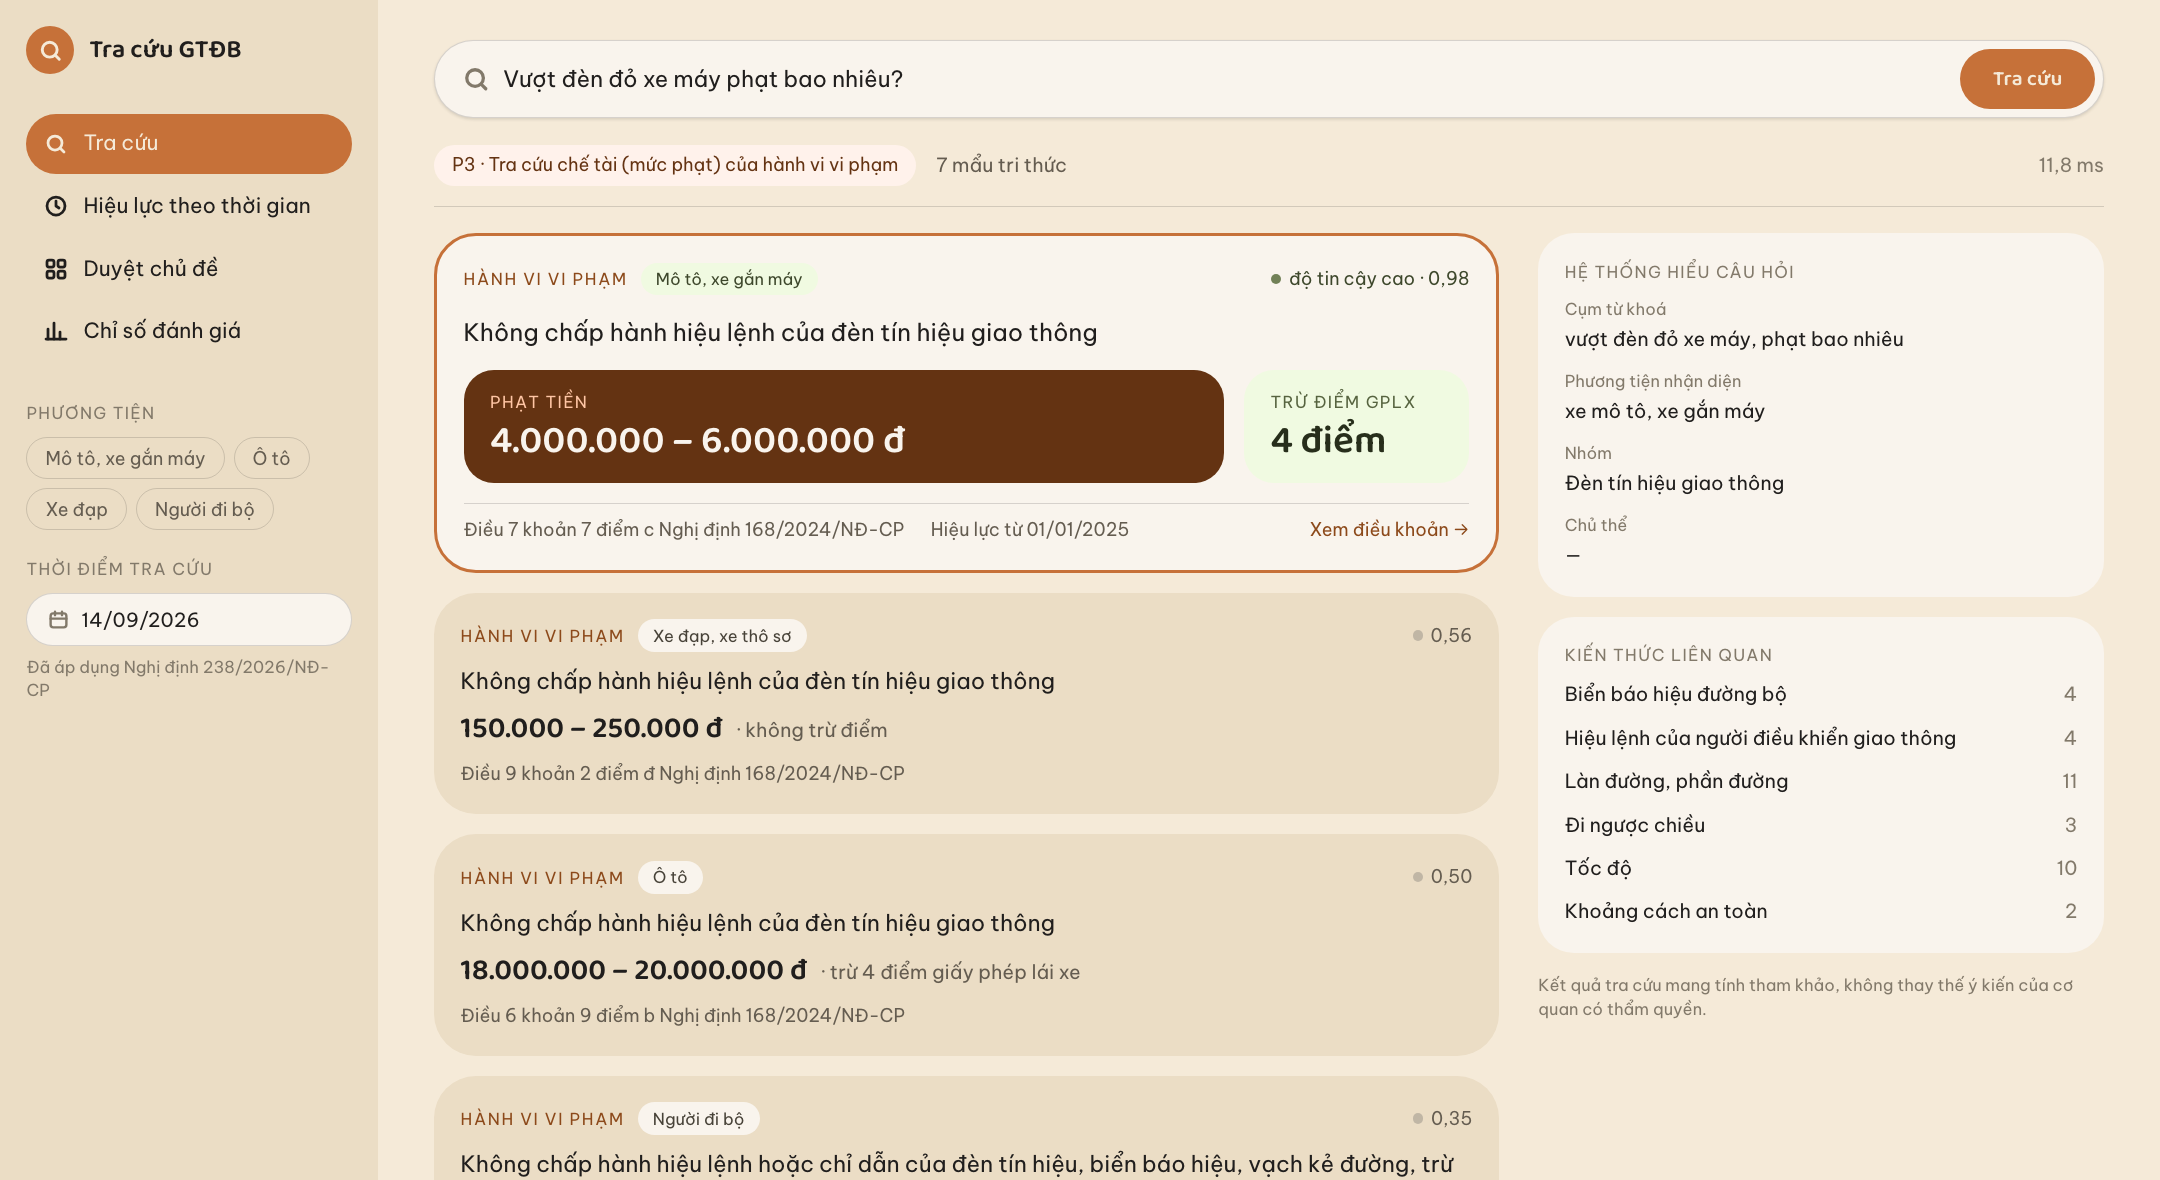
\includegraphics[width=0.97\textwidth]{figures/ui_tra_cuu.png}}
\caption{Màn hình tra cứu với câu hỏi ``Vượt đèn đỏ xe máy phạt bao nhiêu?'': kết quả hạng 1
đúng khung Điều 7 khoản 7 điểm c NĐ 168/2024, kèm mức phạt, điểm trừ GPLX, căn cứ và phần
``hệ thống hiểu câu hỏi'' (cụm từ khoá, phương tiện, nhóm)}
\label{fig:ui-tra-cuu}
\end{figure}

\begin{figure}[H]
\centering
\fbox{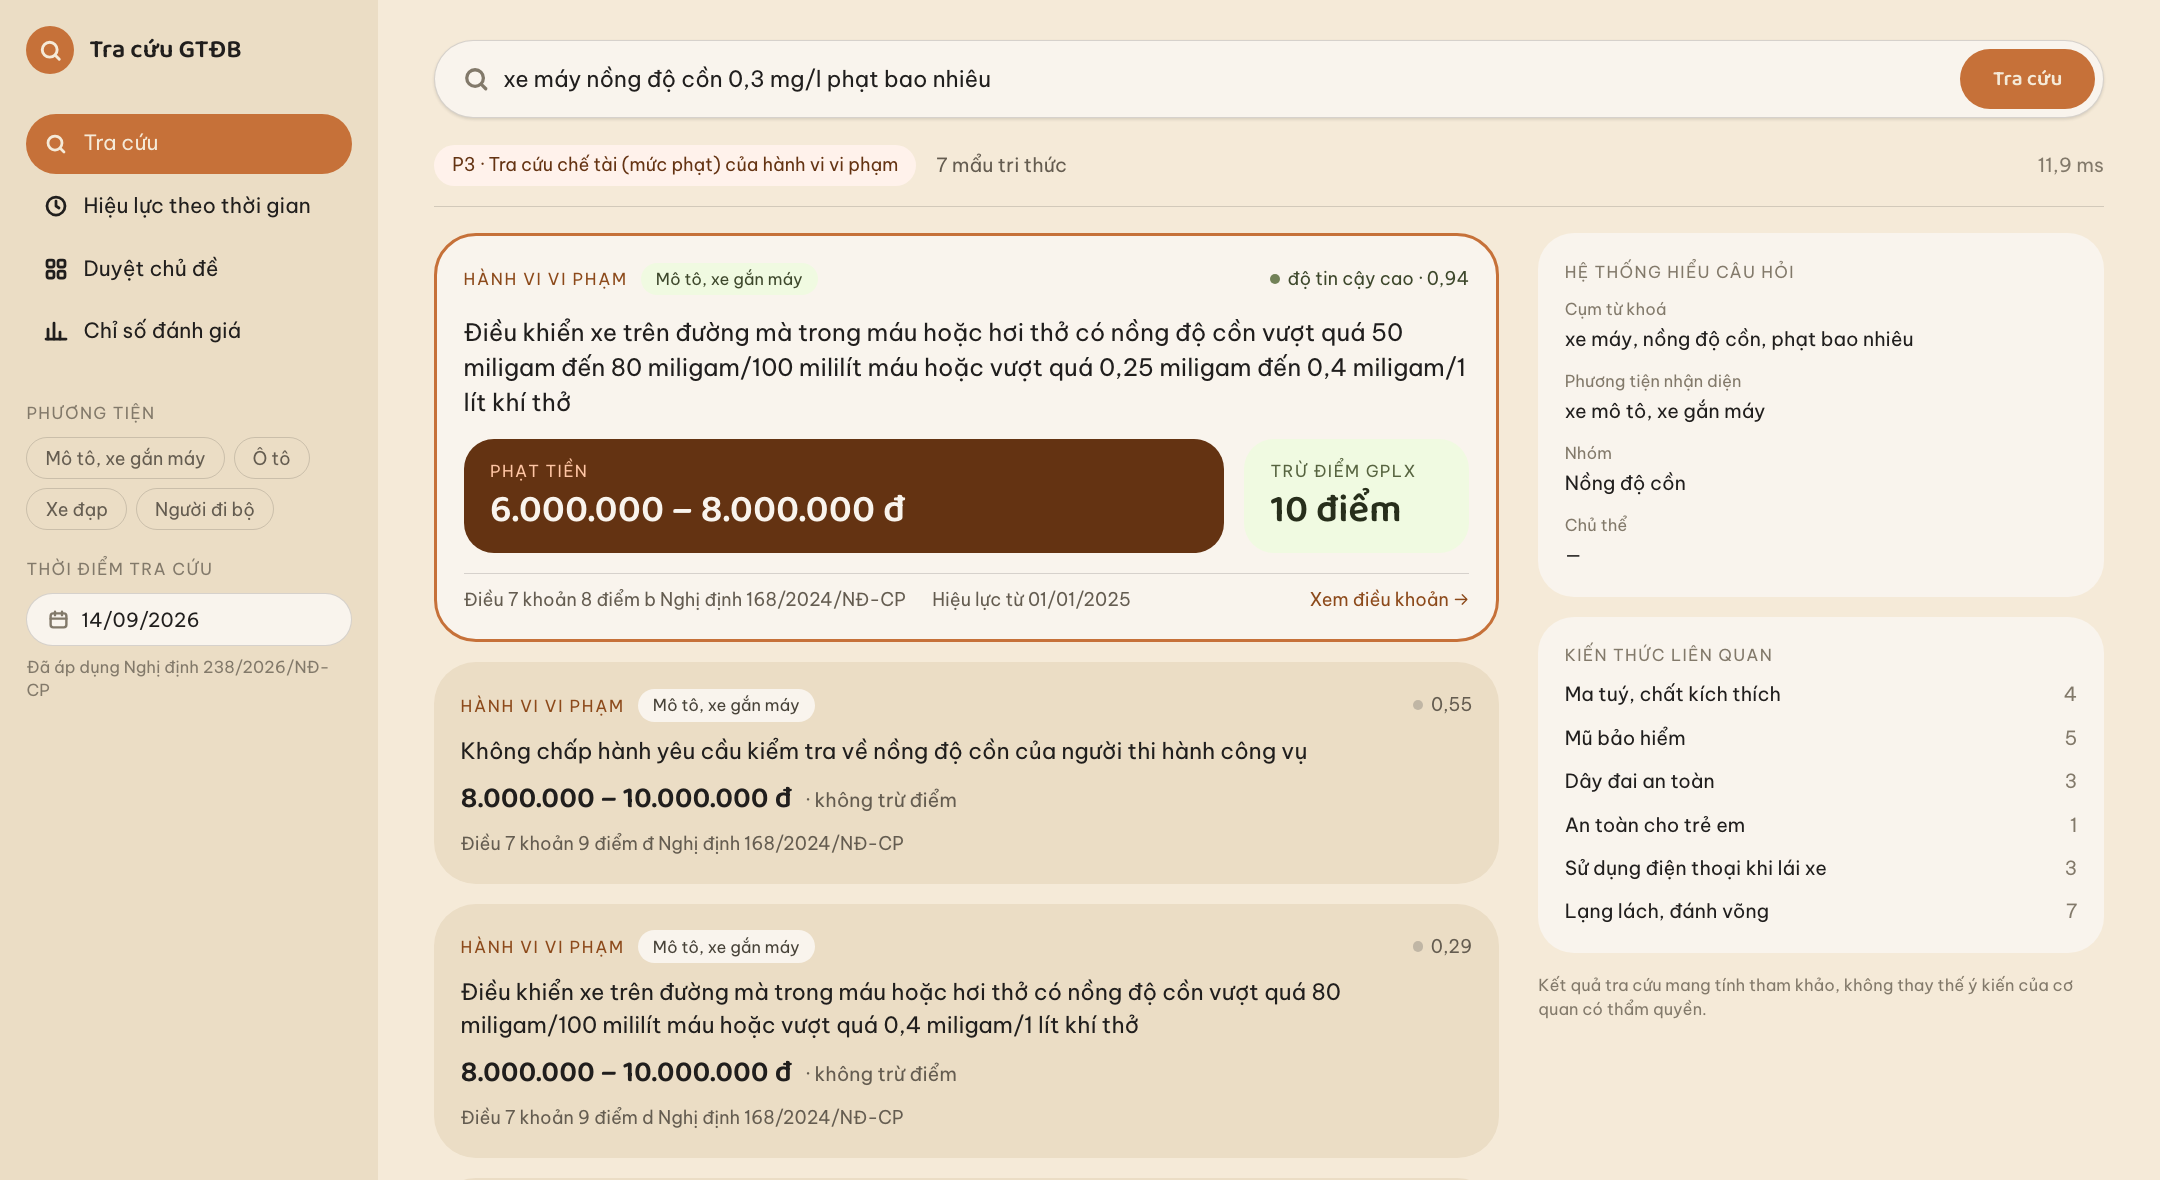
\includegraphics[width=0.97\textwidth]{figures/ui_so_hoc.png}}
\caption{Suy diễn số học: với ``xe máy nồng độ cồn 0,3 mg/l'', khung ``vượt quá 0,25 đến 0,4
miligam/1 lít khí thở'' (6--8 triệu đồng, trừ 10 điểm) được đẩy lên đầu}
\label{fig:ui-so-hoc}
\end{figure}

\begin{figure}[H]
\centering
\fbox{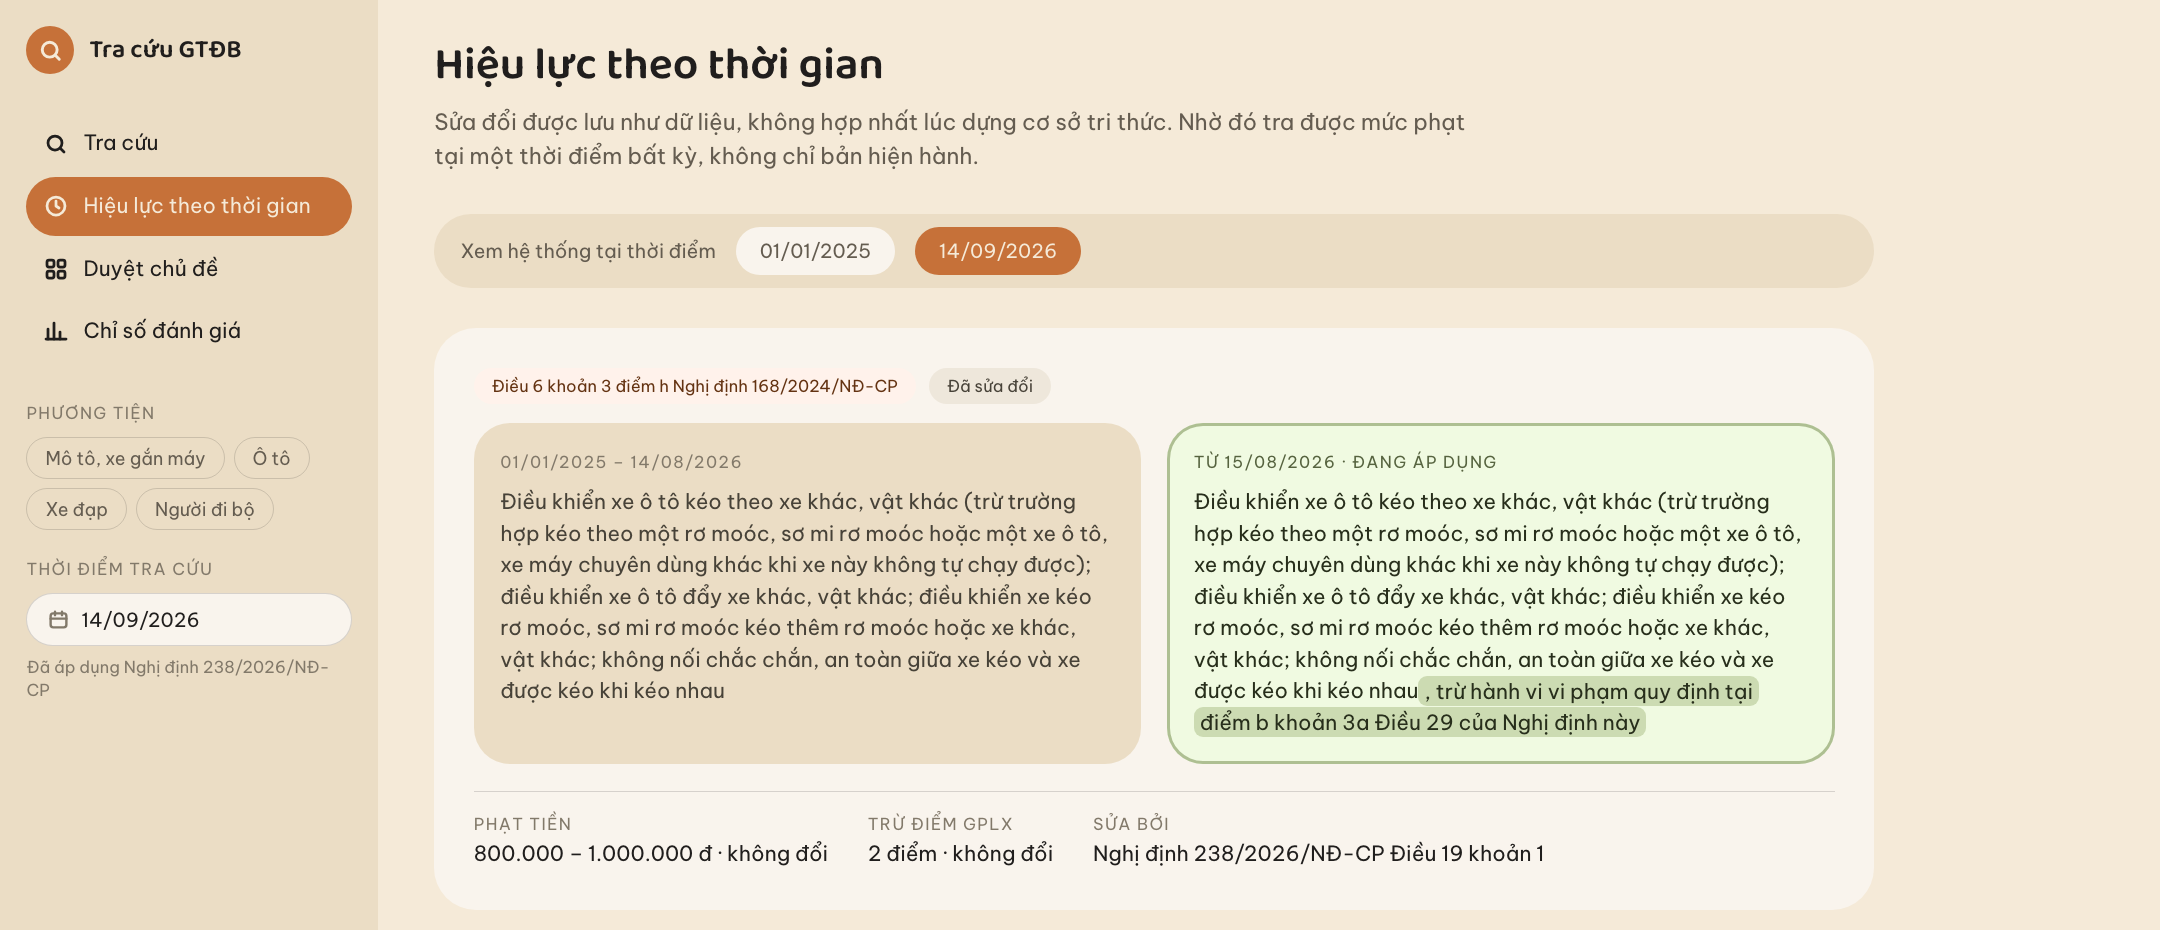
\includegraphics[width=0.97\textwidth]{figures/ui_hieu_luc.png}}
\caption{Màn hình hiệu lực theo thời gian: đối chiếu nguyên văn một điều khoản trước và sau
khi Nghị định 238/2026/NĐ-CP có hiệu lực (15/8/2026)}
\label{fig:ui-hieu-luc}
\end{figure}

Giá trị sử dụng thực tế nằm ở ba chỗ: câu trả lời luôn kèm căn cứ tới mức điều -- khoản -- điểm
nên kiểm chứng được; tra cứu được theo mốc thời gian nên không đưa nhầm quy định đã hết hiệu
lực; và toàn bộ chạy cục bộ trong khoảng 6~ms mỗi truy vấn, không gửi câu hỏi của người dân ra
dịch vụ ngoài.

\subsection{Hạn chế}
\label{sec:han-che}

Mọi hạn chế dưới đây đều đã \textbf{đo được} và phần lớn được khoá lại bằng test \code{xfail}
trong kho mã, không phải phỏng đoán. Nhóm trình bày cả những hướng đã thử và đã bác bỏ, vì một
kết quả âm có số đo cũng là kết quả.

\subsubsection{Chưa từ chối được truy vấn ngoài lĩnh vực}

Ở cấu hình mặc định, hỏi ``cách nấu phở bò'' thì hệ thống vẫn trả về tri thức giao thông: cả
\textbf{40/40} truy vấn ngoài miền đều được trả lời thay vì bị từ chối. Nguyên nhân đã khoanh
vùng: đặc trưng TF-IDF quá yếu để tách miền --- 56/120 câu hợp lệ chấm điểm thấp hơn hoặc bằng
truy vấn rác, nên không tồn tại ngưỡng nào tách được hai phân bố.

\begin{table}[H]
\centering
\caption{Khả năng tách miền của bốn tín hiệu (120 câu trong miền · 40 truy vấn ngoài miền)}
\label{tab:tach-mien}
\renewcommand{\arraystretch}{1.2}
\begin{tabularx}{\textwidth}{@{}L r r r@{}}
\toprule
\textbf{Tín hiệu} & \textbf{AUC} & \textbf{Loại rác khi 0 câu oan} & \textbf{Oan khi loại hết rác} \\
\midrule
TF-IDF thô       & 0,8746 & 7,5\%  & 66,7\% \\
Số keyphrase     & 0,9500 & 0,0\%  & 10,0\% \\
Phủ từ vựng KB   & 0,7243 & 47,5\% & 100,0\% \\
\textbf{Dense embedding} & \textbf{0,9958} & \textbf{77,5\%} & \textbf{5,8\%} \\
\bottomrule
\end{tabularx}
\end{table}

Nhóm đã kiểm chứng đề xuất thay đặc trưng: dense embedding nâng AUC từ 0,8746 lên 0,9958 và
riêng điểm dense loại được 77,5\% truy vấn rác mà không từ chối oan câu hợp lệ nào; bộ lọc kết
hợp keyphrase + dense (ngưỡng 0,45) loại được 92,5\%. Nhưng hai phân bố \emph{vẫn} chồng lấn:
trần điểm dense của truy vấn rác (0,5158) cao hơn sàn điểm của câu hợp lệ (0,3919). Muốn loại
100\% truy vấn rác thì phải chấp nhận từ chối oan 5,8\% câu hợp lệ. Nhóm từ chối đánh đổi đó và
giữ tầng dense ở dạng tuỳ chọn --- mô hình nặng khoảng 470~MB cũng là một lý do. Bản demo mặc
định vì vậy chưa có bộ lọc miền.

\emph{Kết quả âm đáng ghi nhận:} phủ từ vựng cơ sở tri thức là tín hiệu vô dụng cho việc tách
miền (AUC 0,7243, thấp hơn cả TF-IDF thô). Hướng này đã thử và đã bác bỏ.

\subsubsection{Các hạn chế còn lại}

\begin{itemize}
  \item \textbf{Khoảng trống từ vựng là nguồn lỗi lớn nhất:} 15 ca được quy trực tiếp về nguyên
        nhân này, và tính rộng ra thì 27/31 ca chưa tối ưu đều có đặc điểm chung là không cụm từ
        khoá nào của đáp án xuất hiện trong câu hỏi. Đây là hạn chế của dữ liệu chứ không của
        thuật giải.
  \item \textbf{Chưa có tập đánh giá giữ lại:} trọng số hàm điểm được chọn bằng ablation trên
        chính 120 câu hỏi đánh giá, và cổng CI cũng đo trên bộ này. Con số 76,67\% vì vậy là kết
        quả trên bộ câu hỏi dùng trong quá trình phát triển; khả năng khái quát sang câu hỏi mới
        chưa được đo.
  \item \textbf{Bộ câu hỏi chưa phủ đều cơ sở tri thức:} 120 câu chạm tới 115/527 mục tri thức
        truy hồi được (21,8\%); lĩnh vực ``Điều kiện của phương tiện'' bị đánh giá nhẹ hơn tỉ
        trọng của nó.
  \item \textbf{Câu tình huống nhiều vi phạm:} hệ tìm đủ mọi vi phạm ở 9/15 câu P5, nên tổng mức
        phạt có thể thiếu một hành vi.
  \item 12/120 câu hợp lệ không rút được keyphrase nào, nên không thể dùng riêng tín hiệu
        keyphrase làm bộ lọc truy vấn ngoài lĩnh vực.
  \item Chưa mô hình hoá 46 chú thích sửa đổi của Luật 118/2025/QH15 ở mức từng khoản: đã trích
        ra \code{data/raw/luat118\_dieu7\_chu\_thich.json}, nhưng mô hình \code{SuaDoi} hiện chỉ có
        trường theo Nghị định 168 nên chưa biểu diễn được sửa đổi ở tầng luật.
  \item \textbf{Hệ thống không sinh ngôn ngữ tự nhiên:} câu trả lời được ghép từ nguyên văn điều
        khoản. Đây là lựa chọn có chủ đích --- như các số đo ảo giác ở mục~\ref{sec:lien-quan}
        cho thấy, diễn giải lại lời của luật là rủi ro lớn hơn lợi ích về trải nghiệm.
  \item Hỏi nồng độ cồn mà không nêu phương tiện thì hệ trả về khung xe đạp. Về mặt tri thức là
        đúng --- hệ không bịa phương tiện người dùng chưa nói --- nhưng là vấn đề trải nghiệm cần
        giải quyết bằng câu hỏi làm rõ.
  \item Cỡ mẫu 120 câu khiến khoảng tin cậy của các lớp nhỏ rất rộng (P7 với $n = 5$ có KTC
        Top-1 [12\% -- 77\%]), nên không kết luận mạnh được ở mức từng lớp.
\end{itemize}

\subsection{Hướng phát triển}
\label{sec:huong-phat-trien}

\begin{enumerate}
  \item Mở rộng từ điển cụm từ khoá bằng khẩu ngữ thu từ truy vấn thật --- nhắm thẳng vào nhóm lỗi
        L5, nhóm chiếm 15/31 ca chưa tối ưu và là hướng cải thiện rẻ nhất.
  \item Xây một tập câu hỏi giữ lại do người ngoài nhóm soạn, không dùng để chỉnh trọng số, và
        công bố Top-1 trên tập này cạnh con số hiện tại.
  \item Bổ sung tầng hỏi lại khi truy vấn thiếu thông tin bắt buộc (phương tiện, chủ thể) thay vì
        mặc định chọn khung rộng nhất; tách câu tình huống thành từng hành vi trước khi tra.
  \item Thêm tín hiệu phân biệt cho lớp P2: các quy tắc gần nghĩa cần được tách bằng quan hệ trong
        đồ thị $R$, không chỉ bằng điểm tương đồng văn bản.
  \item Tổng quát hoá mô hình \code{SuaDoi} để biểu diễn được sửa đổi ở cả tầng luật và tầng nghị
        định, khép nốt 46 chú thích còn lại --- bước tiến gần hơn tới mô hình sửa đổi hình thức
        của Governatori và cộng sự~\cite{governatori}.
  \item Đưa tầng dense embedding vào bản triển khai có tài nguyên, kèm ngưỡng hai mức: từ chối
        khi chắc chắn, cảnh báo thay vì chặn khi nghi ngờ.
  \item Về dài hạn, công bố cơ sở tri thức và bộ câu hỏi như một tài nguyên mở cho lĩnh vực giao
        thông đường bộ Việt Nam.
\end{enumerate}

\subsection{Kết luận}

Nhóm đã xây dựng hoàn chỉnh một hệ tra cứu kiến thức pháp luật giao thông đường bộ theo đúng
yêu cầu Đề tài 4: cơ sở tri thức có cấu trúc gồm 73 khái niệm, 482 quan hệ, 109 quy tắc, 345
hành vi vi phạm và 1.674 cụm từ khoá; bộ dữ liệu 120 câu hỏi có đáp án chuẩn; thuật giải xử lý
truy vấn sáu bước; và một giao diện tra cứu chạy được.

Về số đo, hệ thống đạt độ chính xác phân lớp 95,83\%, Top-1 76,67\% (KTC 95\% [68,3\% --
83,3\%]), Top-5 95,00\% và MRR 0,8384, thời gian trả lời trung bình 6,2~ms trên máy cá nhân,
hoàn toàn không phụ thuộc dịch vụ ngoài. Thí nghiệm loại bỏ thành phần chứng minh từng phần của
hàm điểm đều đóng góp thực chất, và kiểm định McNemar ($p = 0{,}000488$) khẳng định bước suy
diễn số học tạo khác biệt có ý nghĩa thống kê chứ không phải may rủi.

So với các công trình khảo sát ở mục~\ref{sec:lien-quan}, đóng góp riêng của đồ án nằm ở chỗ
ghép được ba thứ vốn tách rời: mô hình tri thức tường minh theo hướng
Legal-Onto~\cite{legalonto}, suy diễn số học để tính chế tài, và mô hình hoá hiệu lực theo thời
gian ở mức khoản --- trên khung pháp lý giao thông đường bộ 2024--2026.

Điều nhóm thấy đáng giá nhất không phải là con số Top-1 mà là \textbf{kỷ luật đo đạc}: mọi
khẳng định trong báo cáo này đều sinh ra từ một lệnh chạy lại được, mọi hạn chế đều có số đo
kèm theo, mọi tỉ lệ đều kèm khoảng tin cậy, và những hướng đã thử rồi bác bỏ đều được ghi lại
thay vì giấu đi.

% ============================================================================
%  TÀI LIỆU THAM KHẢO
%  Ghi chú: bản Word trước đây đánh số trích dẫn trong thân bài lệch 5 so với
%  danh mục (ví dụ PhoBERT được trích là [6] nhưng nằm ở mục 11). Bản LaTeX dùng
%  khoá \cite nên số thứ tự luôn khớp.
% ============================================================================
\clearpage
\phantomsection
\addcontentsline{toc}{section}{Tài liệu tham khảo}
{\small
\begin{thebibliography}{99}
\setlength{\itemsep}{0.15em}

% ---------- Văn bản pháp luật ----------
\bibitem{luat36} Quốc hội (2024). \emph{Luật Trật tự, an toàn giao thông đường bộ} số 36/2024/QH15.
\bibitem{nd168} Chính phủ (2024). \emph{Nghị định 168/2024/NĐ-CP} quy định xử phạt vi phạm hành chính về trật tự, an toàn giao thông trong lĩnh vực giao thông đường bộ.
\bibitem{luat118} Quốc hội (2025). \emph{Luật 118/2025/QH15} sửa đổi, bổ sung một số điều của 10 luật liên quan đến an ninh, trật tự.
\bibitem{nd238} Chính phủ (2026). \emph{Nghị định 238/2026/NĐ-CP} sửa đổi, bổ sung Nghị định 168/2024/NĐ-CP.
\bibitem{vbhn55} Văn phòng Quốc hội (2026). \emph{Văn bản hợp nhất 55/VBHN-VPQH} ngày 23/3/2026.

% ---------- Công trình khoa học ----------
\bibitem{mlqatsr} Luu, S. T., Vo, T., Nguyen, H. và cộng sự (2025). VLSP 2025 MLQA-TSR Challenge: Vietnamese Multimodal Legal Question Answering on Traffic Sign Regulation. \emph{Proceedings of the 11th VLSP Workshop}. arXiv:2510.20381.
\bibitem{vlqa} Nguyen, T.-M., Nguyen, H.-T., Dao, T.-K. và cộng sự (2025). VLQA: The First Comprehensive, Large, and High-Quality Vietnamese Dataset for Legal Question Answering. arXiv:2507.19995.
\bibitem{drill} Vuong, T.-H.-Y., Nguyen, T.-M., Nguyen, H.-T. và cộng sự (2025). DRILL Shared Task 2025: The Challenge of Deep Retrieval in the Expansive Legal Landscape. \emph{VLSP 2025}.
\bibitem{alqac} Nguyen, H. T. và cộng sự (2021). A Summary of the ALQAC 2021 Competition. arXiv:2204.10717.
\bibitem{zalo} Zalo AI Challenge (2021). Legal Text Retrieval --- bộ dữ liệu truy hồi văn bản luật tiếng Việt.
\bibitem{phobert} Nguyen, D. Q., Nguyen, A. T. (2020). PhoBERT: Pre-trained Language Models for Vietnamese. \emph{Findings of EMNLP 2020}. arXiv:2003.00744.
\bibitem{phamMultistage} Pham, N.-M., Nguyen, H.-T., Do, T.-H. (2022). Multi-stage Information Retrieval for Vietnamese Legal Texts. arXiv:2209.14494.
\bibitem{tienSynthetic} Tiên, S., Doan, H., Dai, A., Đinh Việt, S. (2024). Improving Vietnamese Legal Document Retrieval using Synthetic Data. arXiv:2412.00657.
\bibitem{ducRAG} Duc, N. Q., Son, L. H., Nhan, N. D. và cộng sự (2024). Towards Comprehensive Vietnamese Retrieval-Augmented Generation and Large Language Models. arXiv:2403.01616.
\bibitem{coliee} Goebel, R., Kano, Y., Kim, M.-Y. và cộng sự (2024). Overview and Discussion of the Competition on Legal Information, Extraction/Entailment (COLIEE) 2023. \emph{The Review of Socionetwork Strategies}, 18(1), 27--47. DOI: 10.1007/s12626-023-00152-0.
\bibitem{captain} Nguyen, C., Nguyen, P., Tran, T. và cộng sự (2024). CAPTAIN at COLIEE 2023: Efficient Methods for Legal Information Retrieval and Entailment Tasks. arXiv:2401.03551.
\bibitem{nguyenAttentive} Nguyen, H.-T., Phi, M.-K., Ngo, X.-B. và cộng sự (2022). Attentive Deep Neural Networks for Legal Document Retrieval. \emph{Artificial Intelligence and Law}. DOI: 10.1007/s10506-022-09341-8.
\bibitem{legalbert} Chalkidis, I., Fergadiotis, M., Malakasiotis, P. và cộng sự (2020). LEGAL-BERT: The Muppets straight out of Law School. \emph{Findings of EMNLP 2020}. arXiv:2010.02559.
\bibitem{legalonto} Nguyen, T. H., Nguyen, H. D., Pham, V. T., Tran, D. A., Selamat, A. (2022). Legal-Onto: An Ontology-based Model for Representing the Knowledge of a Legal Document. \emph{ENASE 2022}. DOI: 10.5220/0011066300003176.
\bibitem{phamOntoKG} Pham, V. T., Dang, D. V., Ngo, H. Q. và cộng sự (2025). Ontology-Based Knowledge Graph Approach for Legal Queries. \emph{Informatica}. DOI: 10.15388/25-infor617.
\bibitem{dangKG} Dang, D. V., Pham, V. T., Cao, T., Do, N., Ngo, H. Q., Nguyen, H. D. (2024). A Practical Approach to Leverage Knowledge Graphs for Legal Query. \emph{ISDS 2023}, Springer. DOI: 10.1007/978-981-99-7649-2\_21. (Áp dụng cho luật giao thông đường bộ Việt Nam theo Luật 23/2008/QH12.)
\bibitem{phamLegalOntoUpdate} Pham, V. T., Do, H. D. T., Nguyen, T. H. và cộng sự (2025). Improving Legal Document Analysis and Automatic Knowledge Updates with Legal-Onto Ontology. \emph{SN Computer Science}, 6, art. 874. DOI: 10.1007/s42979-025-04432-0.
\bibitem{leIntelligent} Le, H. H., Nguyen, C.-T., Ngo, T. P. và cộng sự (2023). Intelligent Retrieval System on Legal Information. \emph{ACIIDS 2023}, LNCS 13995. DOI: 10.1007/978-981-99-5834-4\_8.
\bibitem{phamLabor} Pham, V., Le, H. H., Ngo, T. P. và cộng sự (2024). Enhancing legal research through knowledge-infused information retrieval for Vietnamese labor law. \emph{IJAI}, 13(4), 3962--3973. DOI: 10.11591/ijai.v13.i4.pp3962-3973.
\bibitem{phamUnified} Pham, V., Phan, M. C., Cao, B. Q. và cộng sự (2026). A Unified Ontology-Based Knowledge Graph Framework for Multi-Domain Vietnamese Legal Document Retrieval. \emph{MJSAT}, 6(2). DOI: 10.56532/mjsat.v6i2.684.
\bibitem{relamodel} Nguyen, H. D., Do, V. N. và cộng sự (2018). Knowledge-Based Model of Expert Systems Using Rela-Model. \emph{International Journal of Software Engineering and Knowledge Engineering}, 28(8). DOI: 10.1142/S0218194018500304.
\bibitem{cokb} Do, V. N. Ontology COKB for Knowledge Representation and Reasoning in Designing Knowledge-Based Systems. Springer. DOI: 10.1007/978-3-319-17530-0\_8.
\bibitem{lkif} Hoekstra, R., Breuker, J., Di Bello, M., Boer, A. (2007). The LKIF Core Ontology of Basic Legal Concepts. \emph{CEUR-WS} Vol. 321 (LOAIT 2007).
\bibitem{legalruleml} Athan, T., Boley, H., Governatori, G. và cộng sự (2013). OASIS LegalRuleML. \emph{ICAIL 2013}; LegalRuleML Core Specification v1.0, OASIS Standard (2021).
\bibitem{dahl} Dahl, M., Magesh, V., Suzgun, M., Ho, D. E. (2024). Large Legal Fictions: Profiling Legal Hallucinations in Large Language Models. \emph{Journal of Legal Analysis}, 16(1). arXiv:2401.01301.
\bibitem{magesh} Magesh, V., Surani, F., Dahl, M. và cộng sự (2025). Hallucination-Free? Assessing the Reliability of Leading AI Legal Research Tools. \emph{Journal of Empirical Legal Studies}. DOI: 10.1111/jels.12413. arXiv:2405.20362.
\bibitem{alce} Gao, T., Yen, H., Yu, J., Chen, D. (2023). Enabling Large Language Models to Generate Text with Citations (benchmark ALCE). \emph{EMNLP 2023}. arXiv:2305.14627.
\bibitem{phamKGRAG} Pham, V., Phan, M. C. (2025). Integrating Knowledge Graph with Retrieval-Augmented Generation for Vietnamese Legal Question Answering. DOI: 10.59232/dst-v5i1p101.
\bibitem{laura} Tran, V.-K., Nguyen, V. (2025). LAURA: A Legal Agent Using Reasoning and Acting for Vietnamese Law. \emph{KSE 2025}. DOI: 10.1109/KSE68178.2025.11309628.
\bibitem{governatori} Governatori, G., Palmirani, M., Riveret, R., Rotolo, A., Sartor, G. Norm Modifications in Defeasible Logic. \emph{JURIX}.
\bibitem{palmirani} Palmirani, M., Ognibene, T., Cervone, L. Legal Rules, Text and Ontologies Over Time. \emph{RuleML} (CEUR-WS Vol. 874).
\bibitem{demartim} de Martim, H. (2025). An Ontology-Driven Graph RAG for Legal Norms: A Structural, Temporal, and Deterministic Approach. arXiv:2505.00039.
\end{thebibliography}
}

% ============================================================================
%  PHỤ LỤC
% ============================================================================
\clearpage
\appendix
\renewcommand{\thesection}{\Alph{section}}
\titleformat{\section}{\normalfont\Large\bfseries}{Phụ lục \thesection.}{0.6em}{}

\section{Phân công công việc}

\begin{table}[H]
\centering
\caption{Phân công bảy thành viên Nhóm 7}
\label{tab:phan-cong}
\renewcommand{\arraystretch}{1.25}
\begin{tabularx}{\textwidth}{@{}l c L@{}}
\toprule
\textbf{Họ và tên} & \textbf{MSSV} & \textbf{Nội dung phụ trách} \\
\midrule
Nguyễn Quang Lâm & 25210289 & Mục 1 --- tổng quan, phát biểu bài toán; trang bìa và định dạng toàn bài \\
Trần Trọng Tấn   & 25210334 & Mục 2 --- khảo sát công trình liên quan, bộ dữ liệu đã có và phân tích khoảng trống \\
Lê Quang Thi     & 25210337 & Mục 3 --- nguồn văn bản, quy trình lấy và chuẩn hoá dữ liệu \\
Vỏ Cẩm Thu       & 25210342 & Mục 3 --- thống kê và phân tích bộ dữ liệu, ba biểu đồ phân bố \\
Nguyễn Trí Toàn  & 26410135 & Mục 4 --- kiến trúc, thuật giải B1--B6, hàm điểm lai và cấu hình siêu tham số \\
Nguyễn Văn Thái  & 26410108 & Mục 5 --- bảng chỉ số, kiểm định thống kê và thí nghiệm loại bỏ thành phần \\
Đỗ Quốc Hoàng    & 26410043 & Mục 5 --- phân tích lỗi sâu; mục 6 --- ứng dụng, hạn chế và demo \\
\bottomrule
\end{tabularx}
\end{table}

\section{Cách kiểm chứng lại số liệu}

Mọi con số trong báo cáo này sinh ra từ các lệnh sau, chạy tại thư mục mã nguồn của đồ án
(\code{ma\_nguon/}):

\begin{lstlisting}
pip install -e '.[dev,web,bao-cao]'
pytest -q --cov                        # 286 passed · 5 xfailed · 4 skipped · phủ 90%
python eval/evaluate.py --gate-top1 0.7667   # Bảng 10, 11
python eval/ablation.py                # Bảng 12, 13
python eval/kiem_dinh.py --ghi         # KTC 95%, McNemar, trần precision, bỏ dấu
python eval/phan_tich_loi.py           # Bảng 14, 15 và Hình 6
python scripts/thong_ke_du_lieu.py     # Hình 1, 2, 3
python eval/kich_ban.py --chi-tiet     # 12/12 ca nghiệm thu (Bảng 16)
python eval/phat_hien_mien.py --dense --ghi  # Bảng 18
\end{lstlisting}

Báo cáo này được biên dịch bằng \code{latexmk -xelatex main.tex} từ thư mục
\code{bao\_cao/bao-cao-latex/}. Ba ảnh chụp giao diện (Hình~\ref{fig:ui-tra-cuu}--\ref{fig:ui-hieu-luc})
chụp trực tiếp từ ứng dụng chạy bằng lệnh \code{uvicorn traffic\_law.api.web:app}.

\vspace{1.5em}
\begin{center}
\small\itshape Kết quả tra cứu của hệ thống mang tính tham khảo, không thay thế ý kiến của cơ quan có thẩm quyền.
\end{center}


\end{document}
